\documentclass[referee,pdflatex,sn-mathphys-num]{sn-jnl}
\usepackage{graphicx}
\usepackage{multirow}
\usepackage{amsmath,amssymb,amsfonts}
\usepackage{amsthm}
\usepackage{mathrsfs}
\usepackage[title]{appendix}
\usepackage{xcolor}
\usepackage{textcomp}
\usepackage{manyfoot}
\usepackage{booktabs}
\usepackage{algorithm}
\usepackage{algorithmicx}
\usepackage{algpseudocode}
\usepackage{listings}

% Set graphics path to the master images folder
\graphicspath{{../images/}}

%%% ADDITIONAL PACKAGES %%%

% etoolbox to get rid of underfull hbox warnings in bibliography
\usepackage{etoolbox}
\apptocmd{\sloppy}{\hbadness 10000\relax}{}{}

% anyfontsize gets rid of a warning in the logfile
\usepackage{anyfontsize}

% siunitx makes it easier to typeset units
\usepackage{siunitx}
\newcommand{\h}{\,\unit{\hour}}
\newcommand{\ph}{\unit{\per\hour}}
\newcommand{\um}{\,\unit{\micro\metre}}
\newcommand{\pums}{\unit{\per\micro\metre\squared}}
\newcommand{\nm}{\,\unit{\nano\mole\per\litre}}

\raggedbottom

\begin{document}

\title[Article Title]{A Computational Model Reveals the Effects of the CLASP Protein on Root Zonation in \emph{A. thaliana}}

\author*[1,2]{\fnm{First} \sur{Author}}\email{iauthor@gmail.com}

\author[2,3]{\fnm{Second} \sur{Author}}\email{iiauthor@gmail.com}
\equalcont{These authors contributed equally to this work.}

\author[1,2]{\fnm{Third} \sur{Author}}\email{iiiauthor@gmail.com}
\equalcont{These authors contributed equally to this work.}

\affil*[1]{\orgdiv{Department}, \orgname{Organization}, \orgaddress{\street{Street}, \city{City}, \postcode{100190}, \state{State}, \country{Country}}}

\affil[2]{\orgdiv{Department}, \orgname{Organization}, \orgaddress{\street{Street}, \city{City}, \postcode{10587}, \state{State}, \country{Country}}}

\affil[3]{\orgdiv{Department}, \orgname{Organization}, \orgaddress{\street{Street}, \city{City}, \postcode{610101}, \state{State}, \country{Country}}}

\abstract{
Variations in the rates of cell division and elongation in the root apical meristem of \emph{A. thaliana} have a significant influence on organ development.
In particular, the plant hormone brassinosteroid promotes cell elongation while the CLASP protein affects cell division by influencing the arrangement of microtubule polymers on the cell membrane.
However, the precise effect of CLASP on organ development remains unknown.
In this paper, we develop a computational model to investigate root zonation in \emph{A. thaliana} mutants where the brassinosteroid/CLASP signalling network has been disrupted.
The model is based on brassinosteroid receptor dynamics and their downstream effects on CLASP, cell division, and cell elongation.
In order to fit our model to data, we find that there must be a maximum rate of cell division at an intermediate concentration of CLASP.
At CLASP concentrations above and below this critical value, our model predicts a lower rate of cell division. This finding suggests that the CLASP protein must be precisely regulated to ensure optimal organ development.
}

\keywords{Brassinosteroid, Cell Division, CLASP, Microtubules, Root Zonation}

\maketitle

\section*{Introduction}\label{sec1}

Environmental stressors such as drought, heat, and cold are known to cause significant changes in the hormone and protein levels of plants \cite{halat2020}.
As a result of these fluctuations in intracellular signalling, plants often undergo profound changes in morphology.
Developing a better understanding of how hormones and proteins interact to drive organ-scale behaviour in plants is essential for the increasingly important field of sustainable agriculture.
One system of interest for studying this phenomenon is the root apical meristem of \emph{A. thaliana}, where the division and elongation of individual cells governs the development of the root.
In the meristem, cells proliferate in a region known as the division zone.
This zone is located directly above the quiescent center—a small cluster of slowly dividing stem cells located at the root tip \cite{verbelen2006}.
Beyond the division zone, cells lose the capacity to divide and instead undergo rapid elongation as they enter the elongation zone.
This developmental transition is essential for proper root growth and is tightly controlled by molecular regulators.
In this paper, we investigate how the CLASP protein and the plant hormone brassinosteroid influence the transition from cell division to cell elongation.

Cell elongation in plants is driven by turgor pressure, the force exerted by intracellular fluid on the plasma membrane.
The organized deposition of cellulose microfibrils on the cell wall creates anisotropic resistance to the uniform turgor pressure, causing the vertical cell elongation observed in the meristem \cite{hamant2010}.
The arrangement of tubulin polymers known as microtubules has been shown to guide cellulose deposition on the cell wall \cite{hamant2010}, although it remains unclear whether this effect is significant enough to drive changes in cell elongation.
The CLASP protein plays an essential role in determining microtubule arrangement by allowing microtubules to cross sharp edges on the cell membrane \cite{ambrose2011}.
This results in the formation of transfacial bundles of microtubules (TFBs) along the transverse and radial edges of the cell \cite{halat2022}.
TFBs are only observed in mitotic cells \cite{ambrose2011}, although it remains unknown whether this relationship is causal \cite{halat2022}. 

Brassinosteroids (BRs) are a class of plant hormone that have been shown to promote cell elongation \cite{ackerman-lavert2020}.
Extracellular BRs, such as the highly potent brassinolide (BL), bind to the receptor BRI1 and its homologues on the cell membrane \cite{vukasinovic2021}.
Bound BRI1 receptors inhibit the negative regulator BIN2, which releases the suppression of the BES1 transcription factor \cite{ackerman-lavert2020}.
Both BL and BES1 concentrations are highest in the proximal region of the meristem due to a high concentration of BR precursors \cite{vukasinovic2021}.
The BES1 transcription factors, which are often used as a proxy for intracellular BR signalling, have been shown to inhibit CLASP production \cite{ruan2018}.
Additionally, CLASP influences BR signalling by promoting the recycling of endocytosed BRI1 receptors \cite{ruan2018}.
Together, these two effects produce a positive-negative feedback loop that helps to maintain homeostasis in the root \cite{ruan2018}.

Modifications to the BR/CLASP signalling network can induce significant changes in root morphology.
The \emph{clasp-1} mutant has a loss-of-function mutation that fully inhibits the production of CLASP \cite{ambrose2007}.
This causes microtubules to form organized transverse arrays (OTAs) instead of TFBs and induces premature exit from the cell cycle \cite{halat2022}.
Because cells in the \emph{clasp-1} mutant divide less frequently than cells in the wild type, the \emph{clasp-1} mutant has longer cells and a shorter root \cite{ambrose2007}.
The \emph{brinCLASPpro} mutant is insensitive to the effects of BR signalling, which releases the inhibition of the CLASP promoter \cite{ruan2018}.
The excess of CLASP in the \emph{brinCLASPpro} mutant promotes the recycling of BRI1 receptors \cite{ruan2018}, which leads to higher concentrations of the BES1 transcription factor.
Higher levels of BR signalling are associated with rapid cell elongation, which may cause the \emph{brinCLASPpro} mutant to develop longer cells relative to the wild type.
Consistent with this expectation, cells in the \emph{brinCLASPpro} mutant are longer than those in the wild type.
However, they remain shorter than cells in the \emph{clasp-1} mutant.
Additionally, the \emph{brinCLASPpro} root is shorter than the wild type but longer than the \emph{clasp-1} root.

In this paper, we study the BR/CLASP signalling network (see Figure \ref{network}) using a system of time-dependent ordinary differential equations (ODEs).
By fitting the solutions of these ODEs to experimental data, we show that our current understanding of the BR/CLASP signalling network cannot differentiate the wild type from the \emph{brinCLASPpro} mutant.
Then, we discuss biologically motivated adjustments to our model for recovering the \emph{brinCLASPpro} mutant.
Ultimately, we find strong evidence that the CLASP protein reverses its influence, inhibiting cell division at superphysiological concentrations.
We speculate on the biological mechanisms that drive this phenomenon and suggest avenues for further \emph{in-vivo} and \emph{in-silico} research.


\begin{figure}
\centering
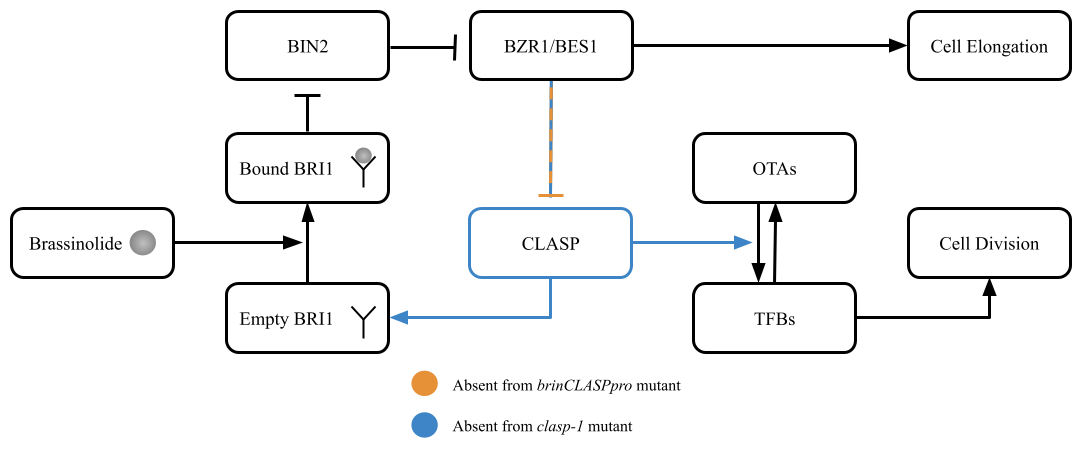
\includegraphics[width=\textwidth]{network-complete.png}
\caption{Known effects of BR and CLASP signalling on cell elongation and division in the meristem of \emph{A. thaliana}. Pointed arrows denote promotion, while flat arrows denote inhibition.
Components of the signalling network that are removed in the \emph{brinCLASPpro} and \emph{clasp-1} mutants are indicated in orange and blue respectively.
 L molecules bind to empty BRI1 receptors to create bound BRI1 receptors, which release the inhibition of the BES1 transcription factor through BIN2.
The BES1 transcription factor inhibits the CLASP promoter and promotes cell elongation.
The CLASP protein promotes the recycling of endocytosed BRI1 receptors and induces the formation of TFBs on the cell membrane.
TFBs are closely linked with cell division, although the exact mechanism by which they influence each other remains unknown. }
\label{network}
\end{figure}

\section*{Methods}\label{sec11}

The length of trichoblast cells in the epidermal columns and their positions relative to the quiescent centre were estimated in the wild type, \emph{brinCLASPpro}, and \emph{clasp-1} lines as described in Appendix \ref{secA1} (see Figure \ref{data-binned}).
Atrichoblast cells were also analyzed but exhibited lesser differences between the wild type and mutant lines so we fit the model to both datasets separately. 
The analysis of the trichoblast data is reported in the Results section and the analysis of the atrichoblast data is reported in Appendix \ref{secA4}.

\begin{figure}
\centering
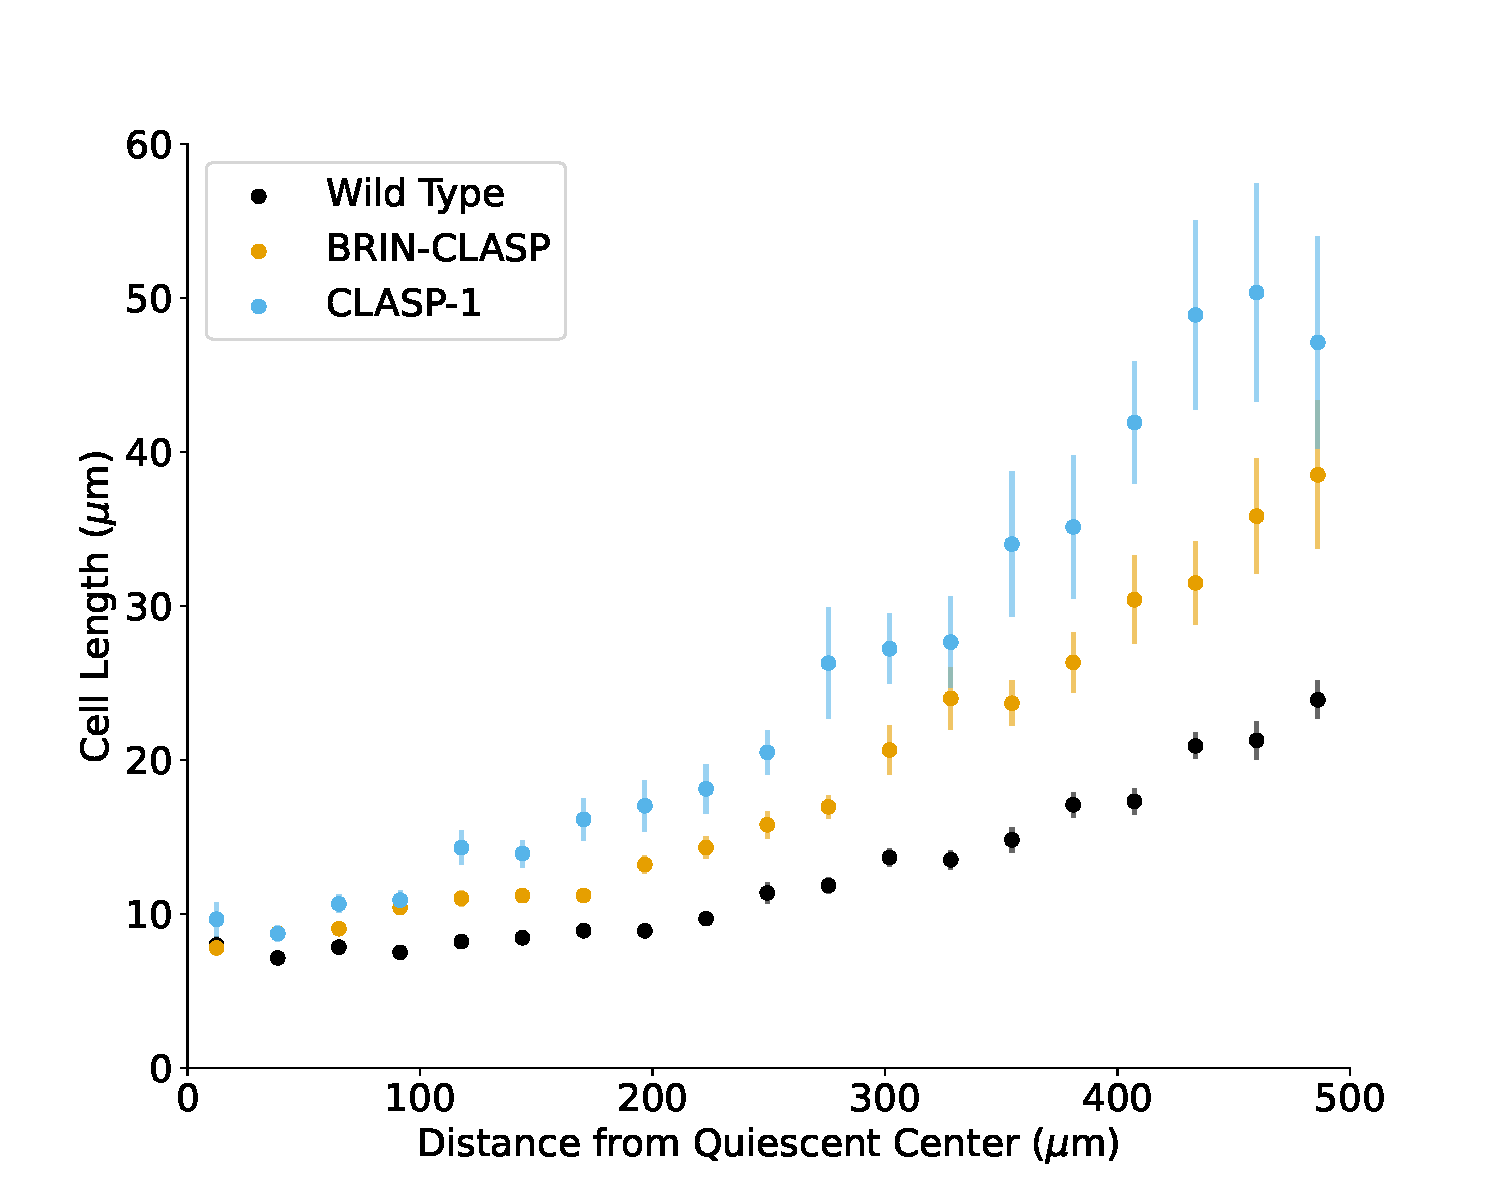
\includegraphics[width=\textwidth]{data-binned-500.pdf}
\caption{Mean cell lengths in the root apical meristem as a function of distance from the quiescent center.
Precisely, each point represents the mean length of the cells whose bottom edge lies within a $25\um$ bin.
In all \emph{A. thaliana} lines, cell length increases as a function of distance from the quiescent center.
Therefore, binning the data yields additional variance because a cell with its bottom edge at $z = 30\um$ will, on average, be shorter than a cell at $z = 40\um$.
However, both of these cells will be counted in the same bin ($25\um$ to $50\um$).
Error bars denote the standard error of the mean $\hat{\sigma}_{x}^{-} = \sigma_{x} / \sqrt{n}$, where $\sigma_{x}$ is the sample standard deviation and $n$ is the number of samples in the bin.
The cells of the \emph{clasp-1} mutant are the largest in all positions shown, followed by the \emph{brinCLASPpro} mutant and then the wild type.
These differences are statistically significant.}
\label{data-binned}
\end{figure}

Our model of the BR/CLASP signalling network in \emph{A. thaliana} consists of two components, a model of intracellular signalling and a model of cell division and growth (the ``cell column model'').
The intracellular signalling model describes the concentrations of CLASP $C$, bound BRI1 receptors $R_{B}$, and total BRI1 receptors $R_{T}$.
This model assumes that the BRI1 receptor system is governed by the mass balance equations proposed by van Esse et al. \cite{vanesse2012}.
Under these assumptions, free BL ligands bind to free BRI1 receptors at a rate of one ligand to one monomer.
The total concentration of BL ligands $B(z)$ is an increasing function of cell distance from the quiescent center $z$, so $C$, $R_{B}$, and $R_{T}$ are implicitly functions of $z$.
Ligand-receptor complexes dissociate at a rate $K_{d}$ which has been estimated in the literature \cite{wang2001, cano-delgado2004}.
Using the mass-balance equations, we can determine $R_{B}$ as a function of $B(z)$, $K_{d}$, and $R_{T}$.

The bound BRI1 receptor concentration $R_{B}$ is coupled with the CLASP concentration $C$ in a positive-negative feedback loop.
First, bound BRI1 receptors promote the transcription of BES1, which we do not model explicitly.
Then, the BES1 transcription factor represses the activity of the CLASP promoter, which reduces the CLASP concentration.
Finally, the CLASP protein promotes the production of new BRI1 receptors, increasing $R_{T}$ and thus $R_{B}$.
Due to computational constraints that arise from coupling the intracellular signalling model to the cell column model, we assume that the cell is in a quasi-steady state. 
Therefore, we can define $C$ and $R_{B}$ as functions of cell position through $B(z)$.
Additionally, we nondimensionalize $C$ such that $C=1$ is the average CLASP concentration in the wild type root and use experimental data from the literature to further simplify our system.
Equation \ref{intracellular-final} shows the final system of equations used in the intracellular signalling model. 
In total, the system has three parameters: $\beta_{0}$, $\beta_{1}$, and $K_{d}$. 
For a detailed derivation of these equations along with a list of assumptions and their sources, see Appendix \ref{secA2}.

\begin{equation}
\label{intracellular-final}
\begin{aligned}
  C(z) &= \beta_{0} - \beta_{1}R_{B} \\[5pt]
  R_{B}(z) &= \frac{(B + R_{T} + K_{d}) - \sqrt{(B + R_{T} + K_{d})^{2} - 4BR_{T}}}{2} \\[5pt]
  R_{T}(z) &= 62 (0.65 + 0.35 C)
\end{aligned}
\end{equation}

The cell column model describes how cell elongation and cell division are influenced by CLASP and the BES1 transcription factor. 
We assume that the rate of cell elongation is proportional to cell length because longer cells have more vertical surface area for cellulose microfibrils to stretch, tear, and reform.
This assumption has been used previously in the literature \cite{lockhart1965}.
In our model, cells stop elongating at a length of $100\um$  based on the ``sizer'' mechanism proposed by Pavelescu et al., 2016 \cite{pavelescu2016}.
Furthermore, the cell elongation rate is an increasing function of the bound BRI1 receptors $R_{B}$, which we use as a proxy for BES1.
The state of a cell within the cell cycle is represented by $D \in [0, 1]$.  When $D = 1$, the cell divides into two cells of equal length, each with $D = 0$.
Progress in the cell cycle proceeds at a dimensionless rate of $1$, which is increased by CLASP with rate $\delta_{1}$. 
We also assume that a sizer mechanism, represented mathematically as a Hill function, causes cells to stop dividing upon reaching a critical length.
Equation \ref{extracellular-final} contains the system of differential equations used for the cell column model. 

\begin{equation}
\label{extracellular-final}
\begin{aligned}
  \frac{ dL }{ dt } &= \left(\gamma_{0} + \gamma_{1}R_{B}(z)\right)L  \\[5pt]
\frac{ dD }{ dt } &= (1 + \delta_{1}C(z))\left( 1 - \frac{ L^{ n } }{ \delta_{0}^{ n } + L^{ n } } \right) 
\end{aligned}
\end{equation}

\section*{Results}\label{sec2}

\subsection*{Intracellular Signalling}\label{sec21}

We used data from Vukašinović et al. \cite{vukasinovic2021}, to fit the intracellular signalling model shown in Equation \ref{intracellular-final}. 
This model depends on the BL function $B(z)$, which does not have a known functional form.
However, $B(z)$ is known to be an increasing function of position $z$ \cite{vukasinovic2021} such that $B(z) < 1\nm$ \cite{vanesse2012} for $z \in [0\um, 1000\um]$.
To identify the BL function that produced the best fit to the data, we tested the linear, quadratic, and Hill models for $B(z)$ shown in Equation \ref{bl-candidates}.

\begin{equation}
\label{bl-candidates}
\begin{aligned}
  \text{Linear}&: B(z) = \alpha_{0} + \frac{(1 - \alpha_{0})z}{1000} \\[5pt]
  \text{Quadratic}&: B(z) = \alpha_{0} + \frac{(1 - \alpha_{0})z^{2}}{1000^{2}} \\[5pt]
  \text{Hill}&: B(z) = \alpha_{0} + \frac{(1 - \alpha_{0})z^{2}}{\alpha_{1}^{2} + z^{2}}
\end{aligned}
\end{equation}

Since the hill function has one additional degree of freedom through the parameter $\alpha_{1}$, we used the Akaike Information Criterion (AIC) \cite{akaike1974} to account for overfitting.
We also applied the AICc correction \cite{sugiura1978} since the sample size of the data was small relative to the number of parameters.
Solutions to the intracellular signalling equations were found using the computer algebra system \href{https://www.sympy.org/en/index.html}{sympy} and the optimal parameter values were identified using the DIviding RECTangles (DIRECT) global optimization algorithm \cite{jones1993} from the \href{https://docs.scipy.org/doc/scipy/reference/generated/scipy.optimize.direct.html}{scipy} scientific computing package.
Three parameters were fitted for the intracellular signalling equations in addition to either one or two parameters from the candidate $B(z)$ function.
The fitted models and experimental data are shown in Figure \ref{bl-functions} and details about the parameters, errors, and AICc values are contained in Table \ref{bl-fits}.

\begin{figure}
  \centering
  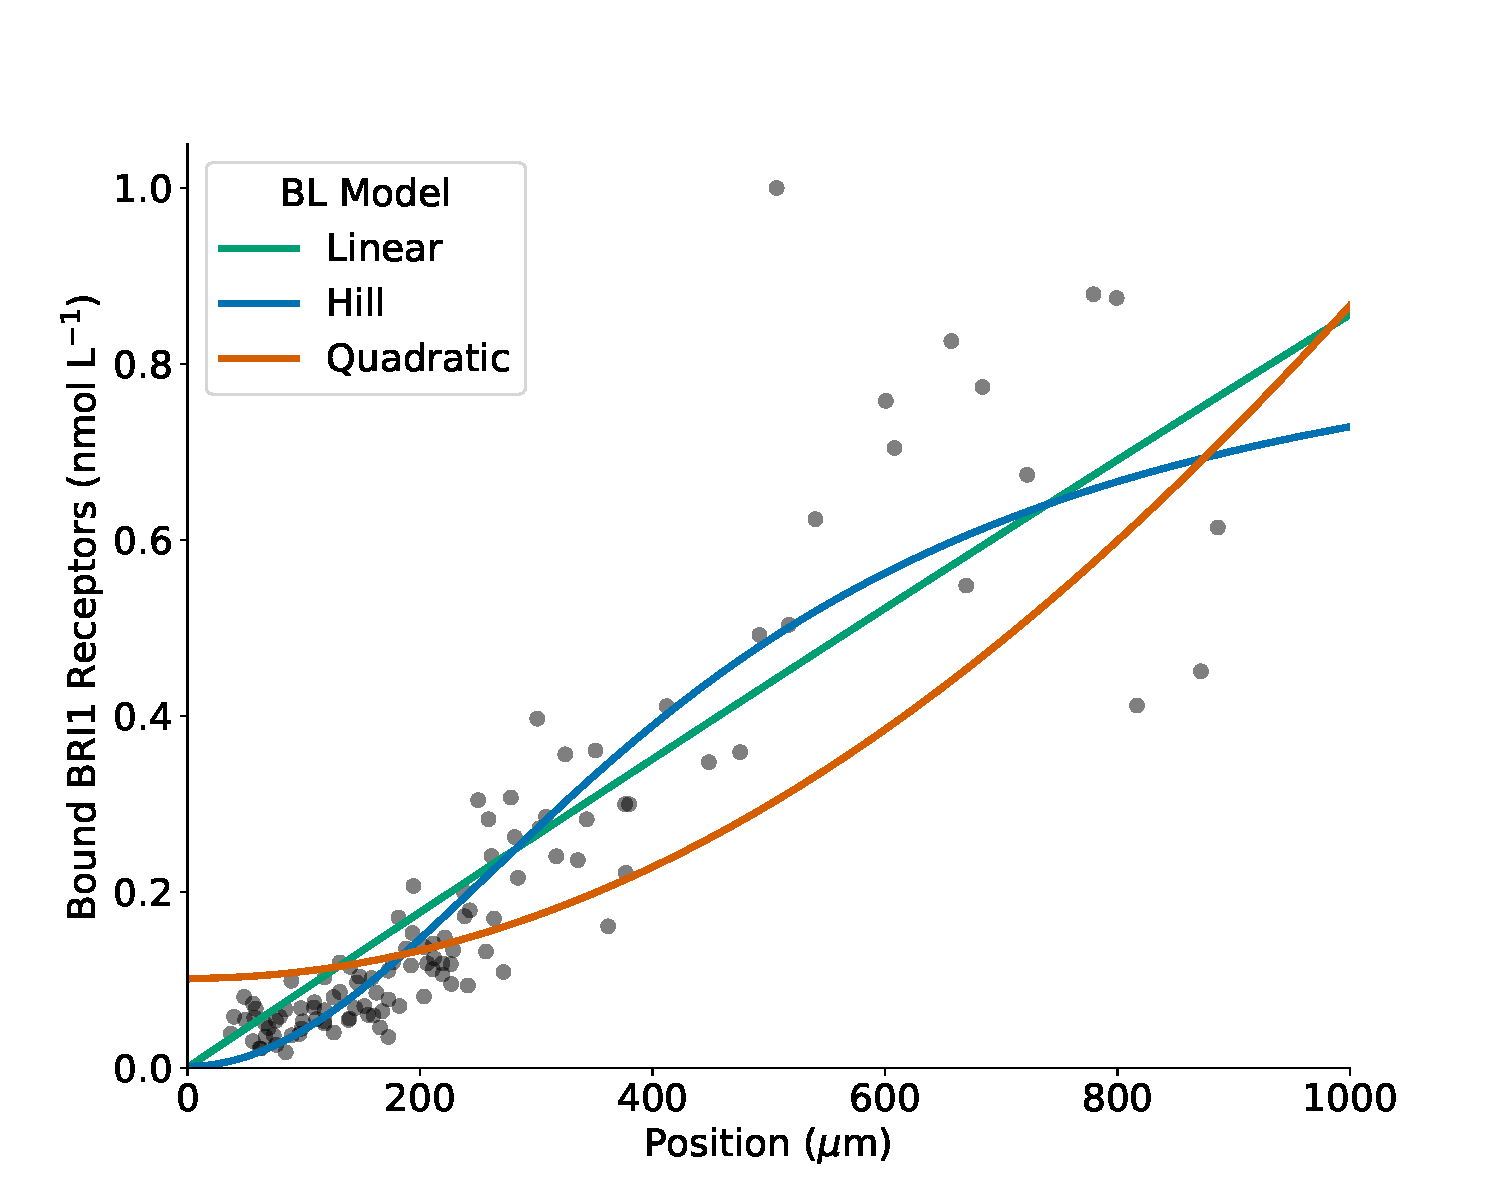
\includegraphics[width=\textwidth]{bes1-functions.pdf}
  \caption{Results of fitting the intracellular signalling equations for CLASP and BRI1 receptor concentrations to experimental data \cite{vukasinovic2021}.
  The Hill model for $B(z)$ yielded the lowest root-mean-squared error (RMSE) at $0.0889$.
The linear model for $B(z)$ had the second lowest RMSE at $0.1000$, followed by the quadratic model for $B(z)$ at $0.1296$.
 }
  \label{bl-functions}
\end{figure}

\begin{table}[ht]
\caption{Details from the linear, hill, and quadratic models for the BL concentration function $B(z)$.
The hill function had the lowest absolute error and the highest AICc value, which suggests that it may be overfitted.
The low variance in the fitted values of the $\beta_{0}$, $\beta_{1}$, and $K_{d}$ parameters between models suggest that our intracellular signalling model is robust to changes in the BL concentration function $B(z)$. }
\label{bl-fits}
\begin{tabular}{@{}llllllll@{}}
\toprule
BL Model & RMSE & AICc & $\alpha_{0}$ & $\alpha_{1}$ & $\beta_{0}$ & $\beta_{1}$ & $K_{d}$ \\
\midrule
Linear & $0.1000$ & $11.694$ & $0.001$ & - & $1.389$ & $0.895$ & $8.901$ \\
Hill & $0.0889$ & $13.685$ & $0.002$ & $456.104$ & $1.389$ & $0.916$ & $7.533$ \\
Quadratic & $0.1296$ & $12.470$ & $0.113$ & - & $1.389$ & $1.08$ & $7.598$ \\
\botrule
\end{tabular}
\end{table}

Since the linear model for $B(z)$ yielded the lowest AICc, we will use this model for subsequent analyses.
Next, we simulated the fitted intracellular signalling model on the \emph{brinCLASPpro} and \emph{clasp-1} mutants by overriding parameter values to modify our \emph{in-silico} signalling network.
To recreate the \emph{clasp-1} mutant we imposed $\beta_{0} = \beta_{1} = 0$ so that $C(z) = 0$. 
Since the \emph{brinCLASPpro} mutant is insensitive to $R_{B}$, we imposed $\beta_{1} = 0$ so that $C(z) = \beta_{0}$.
Notably, we held $\alpha_{0}$ and thus $B(z)$ constant across all three model genotypes.
This decision reflects our assumption that the BL concentration is not modified by the \emph{brinCLASPpro} and \emph{clasp-1} mutations, which may be an oversimplification of the true signalling network.
However, our model still captures the dynamics of the BR/CLASP signalling network shown in Figure \ref{network} by predicting a higher concentration of CLASP and BRI1 receptors in the \emph{brinCLASPpro} mutant and lower concentrations of BRI1 receptors in the \emph{clasp-1} mutant \cite{ruan2018}.
This result is shown in Figure \ref{bes1-mutants}. 

\begin{figure}
  \centering
  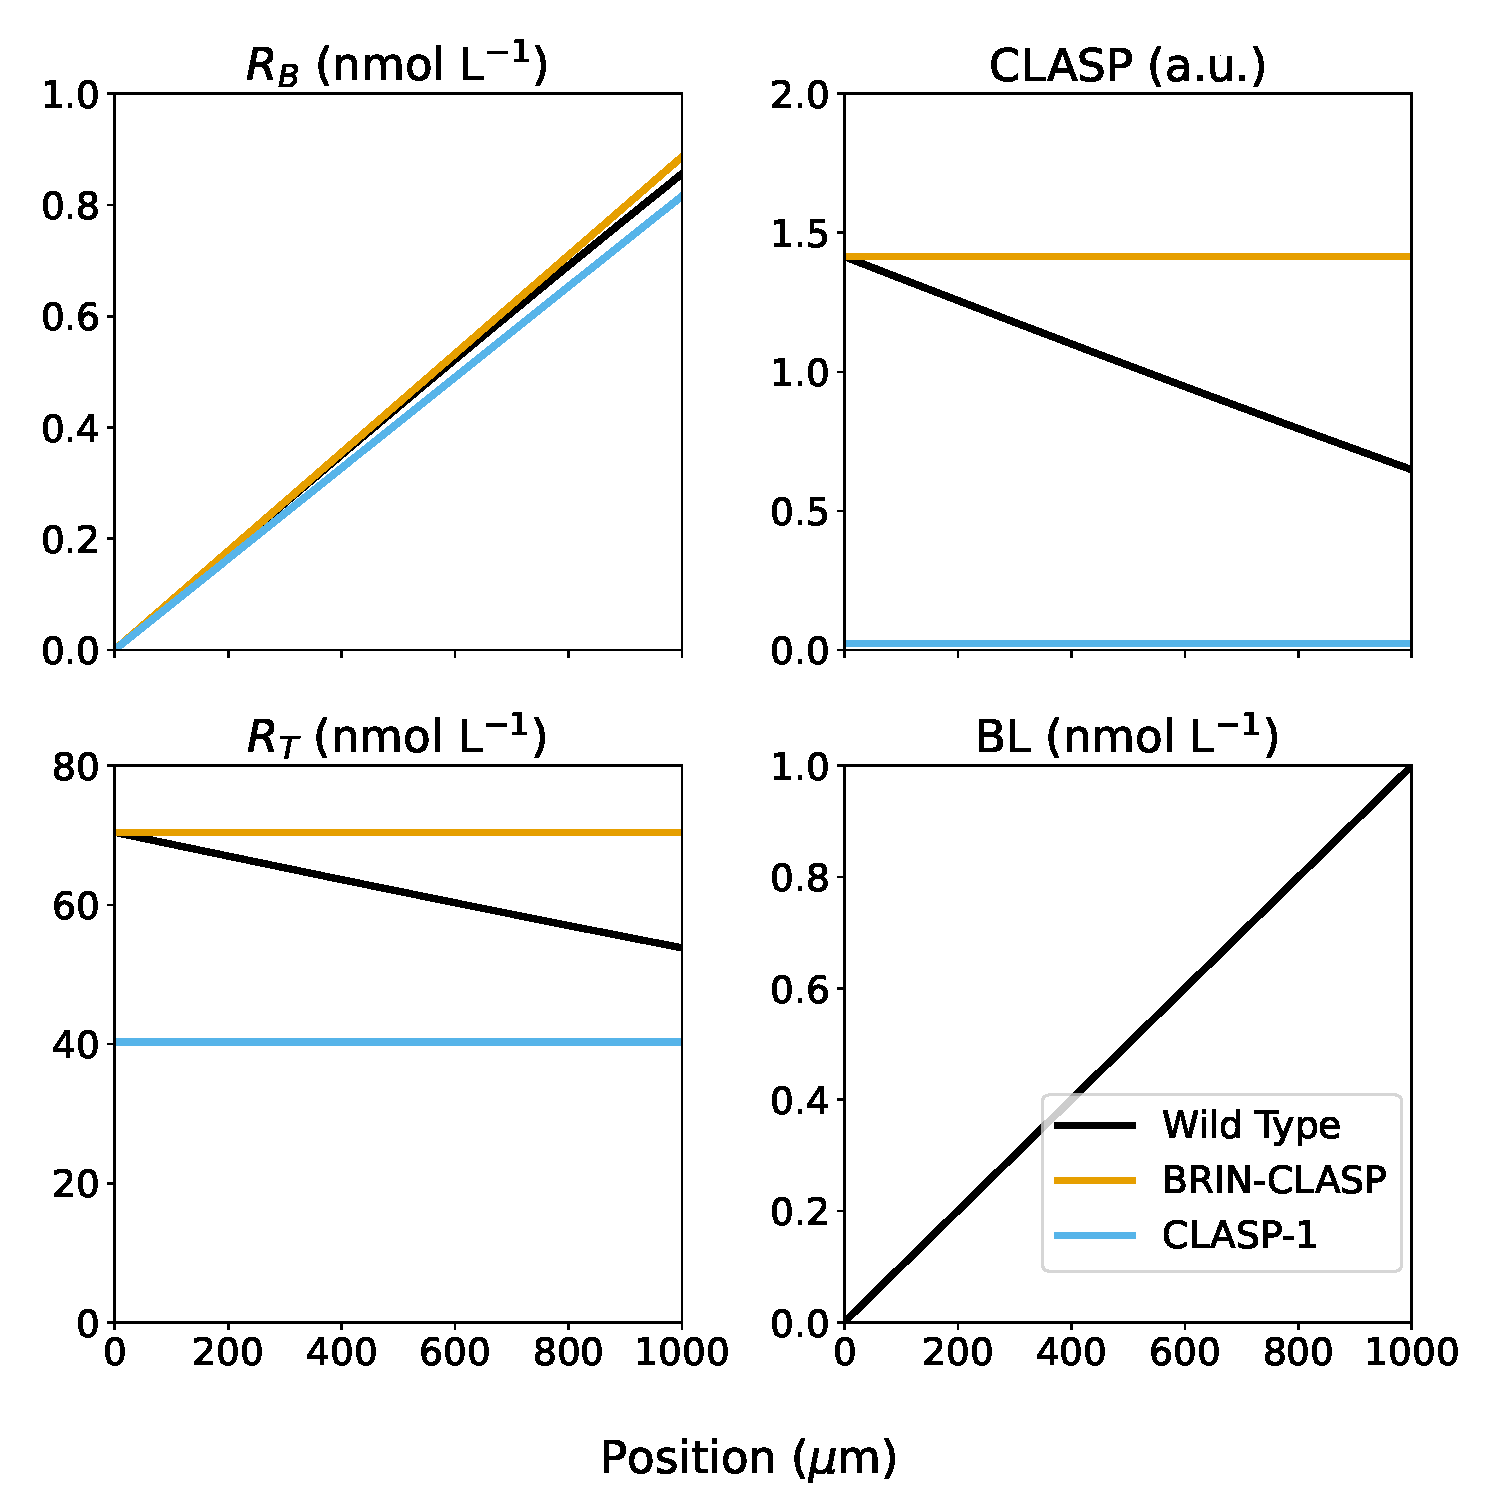
\includegraphics[width=\textwidth]{bes1-mutants.pdf}
  \caption{
Results of simulating the fitted intracellular signalling model on the \emph{brinCLASPpro} and \emph{clasp-1} mutants using the optimal parameters shown in Table \ref{bl-fits}.
The BL function $B(z)$ is assumed to be constant across mutants.
In the \emph{clasp-1} mutant, CLASP is $0$ and BRI1 receptor levels are lower than in the wild type, which reflects our current understanding of the BR/CLASP signalling network.
Conversely, the \emph{brinCLASPpro} mutant exhibits higher levels of CLASP and BRI1 receptors which is also in line with the literature.
  }
\label{bes1-mutants}
\end{figure}

While there is some variance between the bound BRI1 receptor concentrations in the wild type, \emph{brinCLASPpro} mutant, and \emph{clasp-1} mutant, these differences are very small.
This is consistent with previous models \cite{vanesse2012}, which found that no more than $1\%$ of the total BRI1 recpetors were bound.
When $B \ll R_{T}$, the bound BRI1 receptor concentration $R_{B}$ is highly sensitive to changes in the BL concentration $B$ and insensitive to changes in $R_{T}$.
Since the \emph{brinCLASPpro} and \emph{clasp-1} mutants both influence $R_{B}$ through the effect of CLASP on $R_{T}$, it is not surprising that there is little variation in $R_{B}$ between the mutants and the wild type.
Because $R_{B}$ and hence the cell elongation rate $dL/dt$ are effectively constant across all three roots, the differences in cell lengths observed in Figure \ref{data-binned} are likely caused by differences in the cell division rate $dD/dt$.

\subsection*{Cell Columns}

To model the BR/CLASP signalling network at the scale of the entire root, we developed a model of a single column of trichoblast cells in the epidermis from $0\um$ to $500\um$ above the quiescent centre.
The fitted intracellular signalling model is used within the cell column model to calculate the CLASP and BRI1 receptor concentrations as a function of cell position $z$.
Each cell in the cell column model grows and divides based on Equation \ref{extracellular-final}.
An additional parameter $m$, the minimum length of a mitotic cell, was introduced to prevent the formation of unrealistically small cells caused by repeated cell divisions.
Adding $m$ enforces a strict lower bound of $m/2$ on cell length $L$ under our assumptions.
The cell column model was fitted to the experimental data presented in Figure \ref{data-binned} using the DIRECT algorithm \cite{jones1993}.
Model accuracy was evaluated by binning cells by the position of their bottom edge and comparing the mean cell length in each bin to experimental data.
The results of implementing the cell column model are shown in Table \ref{column-fits} and Figure \ref{column-results}.

\begin{table}[ht]
\caption{
Optimal parameter values for the initial cell column model.
$m$, the minimum length of a mitotic cell, was found to be $13.77\um$. 
Since $\gamma_{1} > \gamma_{0}$, cell elongation is primarily driven by BES1 signalling through $R_{B}$.
The fitted Hill function has a half-max of $\delta_{0} = 21.26\um$, which can be interpreted as the maximum length of a mitotic cell.
}
\label{column-fits}
\begin{tabular}{@{}llllllll@{}}
\toprule
RMSE & $m$ & $\gamma_{0}$ & $\gamma_{1}$ & $\delta_{0}$ & $\delta_{1}$ \\
\midrule
$10.401$ & $13.77$ & $0.5247$ & $4.630$ & $21.26$ & $0.2078$ \\
\botrule
\end{tabular}
\end{table}

\begin{figure}
  \centering
  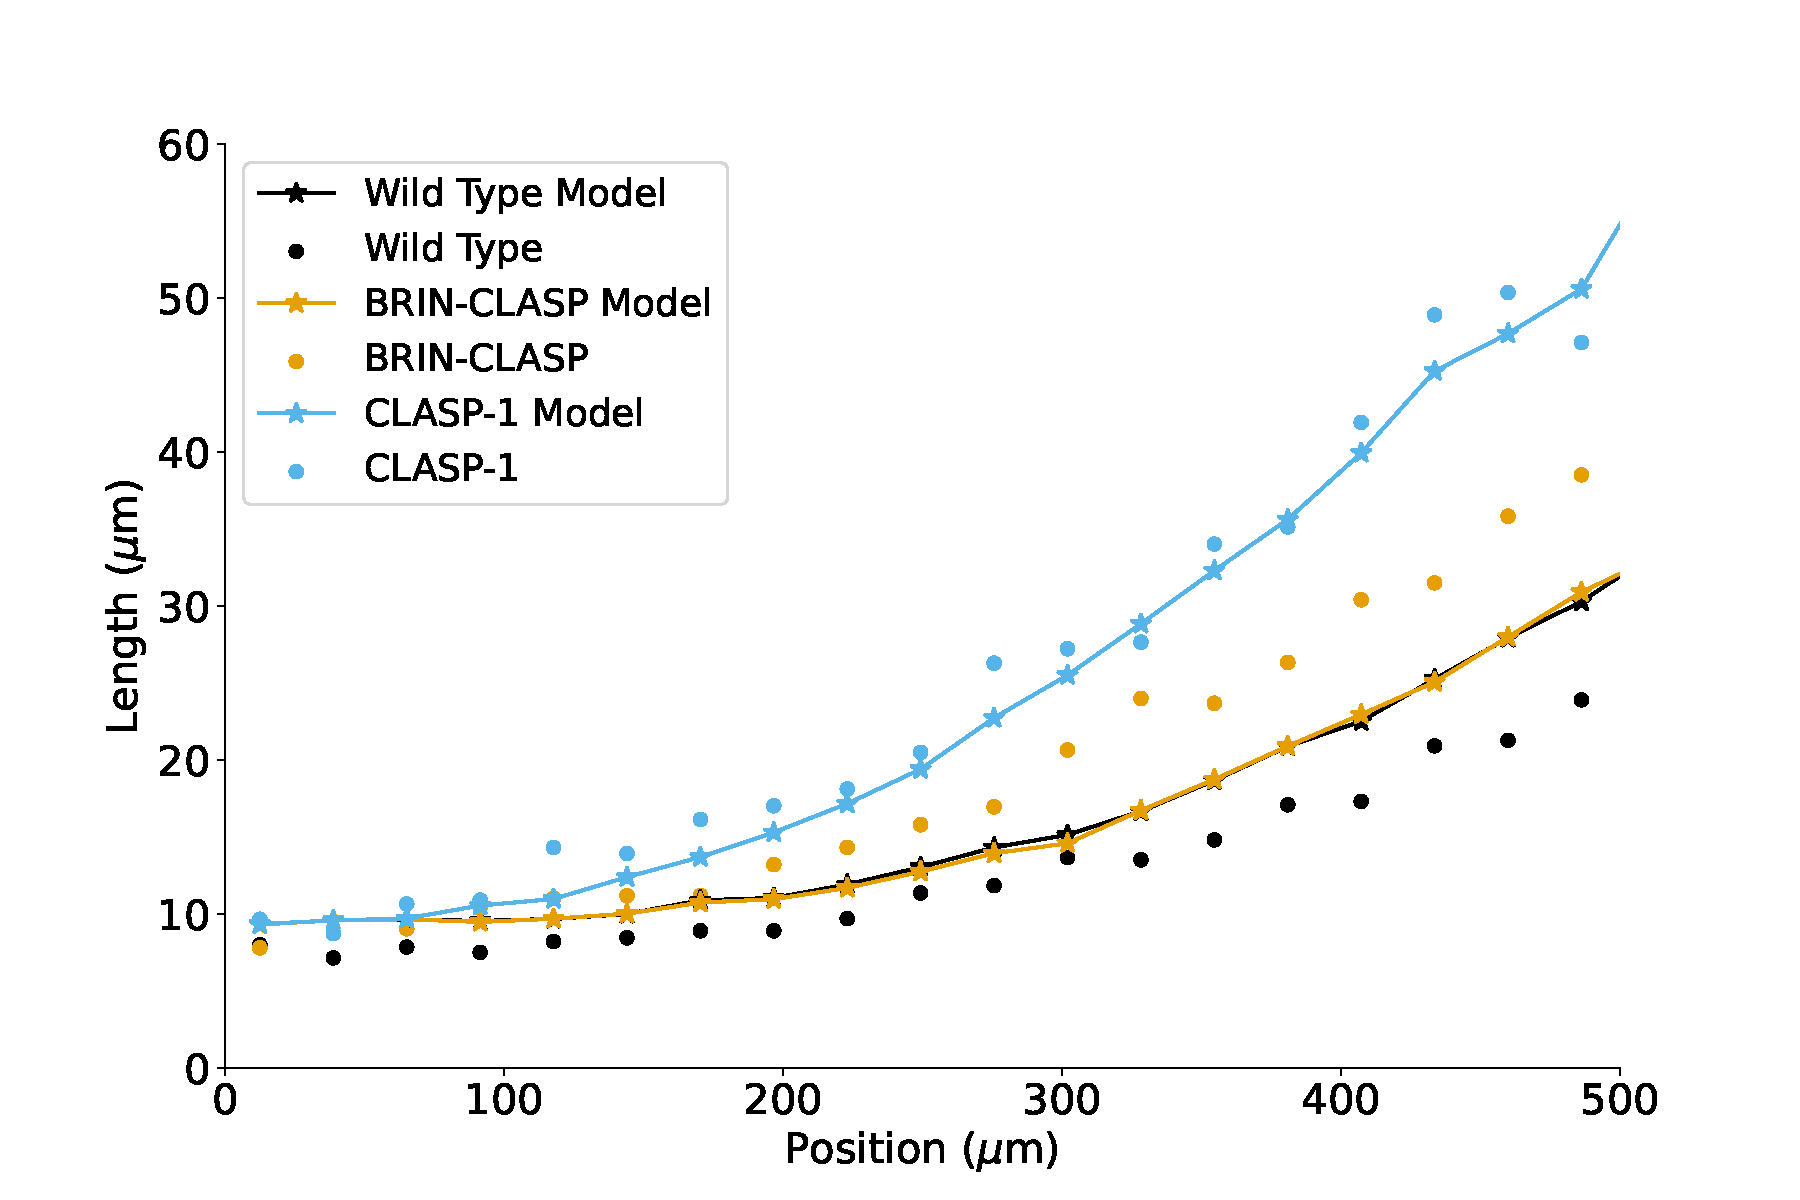
\includegraphics[width=\textwidth]{column-original-fit.pdf}
\caption{Results of fitting the cell column model to experimental data.
The model accurately predicted the behaviour of the \emph{clasp-1} mutant within the standard error of the mean for most positions in the root.
However, the model could not differentiate between the wild type root and \emph{brinCLASPpro} mutant.
This can be observed by the significant overlap between the black and orange markers on the plot above. }
\label{column-results}
\end{figure}

While the fitted model accurately predicted cell lengths in the \emph{clasp-1} mutant, it was unable to differentiate between the wild type and the \emph{brinCLASPpro} mutant.
We believe that the division rate of cells in the \emph{brinCLASPpro} mutant is primarily responsible for this failure, since we previously determined that the rate of cell elongation is roughly constant across genotypes.
Cells in the \emph{brinCLASPpro} root have a higher CLASP concentration than cells in the wild type at the same position due to the lack of inhibition by BES1.
Therefore, cells in the \emph{brinCLASPpro} root must divide more frequently than cells in the wild type, preventing the longer cell lengths observed \emph{in-vivo}.
In conclusion, if we could identify a biological mechanism that decreases $dD/dt$ in the \emph{brinCLASPpro} mutant relative to the wild type, we may be able to achieve a better fit for our model.

\subsection*{Recovering the \emph{brinCLASPpro} Mutant} 

Under our current model, the \emph{brinCLASPpro} mutant has a higher concentration of CLASP which induces a higher rate of cell division relative to the wild type.
However, this phenomenon is not observed \emph{in-vivo}, leading us to speculate that the relationship between CLASP and cell division may be more complicated.
We hypothesize that the CLASP protein stabilizes microtubule polymers until the cell is ready to move to the next phase in the cell cycle.
Therefore, both superphysiological and subphysiological concentrations of CLASP would inhibit cell division.
In the \emph{clasp-1} mutant, which has no CLASP, experimental observations reveal a loose pre-prophase band \cite{ambrose2007} caused by the absence of microtubule rescue.
This malformed pre-prophase band inhibits cell division by slowing down mitosis.
We believe that a related abnormality in the cell cycle causes the lower division rate in the \emph{brinCLASPpro} mutant.
In particular, the superphysiological concentration of the CLASP protein causes an excess of TFBs to form on the cell membrane during interphase.
When the cell enters mitosis, these TFBs must be disassembled in order to make tubulin available for the mitotic spindle. 
This causes cells in the \emph{brinCLASPpro} mutant to divide slower than cells in the wild type.
We model this assumption by modifying the division equation \eqref{division-modified} to include a new parameter $\delta_{2}$.
The re-fitted model under this modification is shown in Figure \ref{column-modified-fit} and Table \ref{column-modified-parameters}.
Ultimately, we find that a cell division function with a maximum rate at an intermediate level of CLASP is sufficient to model the observed cell lengths in the wild type, \emph{clasp-1} and \emph{brinCLASPpro} roots.

\begin{equation}
\label{division-modified}
\frac{dD}{dt} = \left( 1 + \delta_{1} C - \delta_{2} C^{2} \right)\left( 1 - \frac{L^{n}}{\delta_{0}^{n} + L^{n}} \right) 
\end{equation}


\begin{table}[!ht]
\centering
\caption{Optimal parameter values for the fitted cell column model after modifying the division function.
The global maximum of the $dD/dt$ function occurs at $C^{*} = 0.732$.
The minimum length of a mitotic cell was found to be $m = 14.32$.
The fact that $\gamma_{1} > \gamma_{0}$ indicates that the majority of cell elongation is driven by brassinosteroids. }
\label{column-modified-parameters}
\begin{tabular}{@{}llllllll@{}}
\toprule
RMSE & $m$ & $\gamma_{0}$ & $\gamma_{1}$ & $\delta_{0}$ & $ \delta_{1}$ & $\delta_{2}$ \\
\midrule
$5.630$ & $14.32$ & $0.500$ & $4.148$ & $20.26$ & $1.870$ & $1.278$ \\
\botrule
\end{tabular}
\end{table}

\begin{figure}
  \centering
  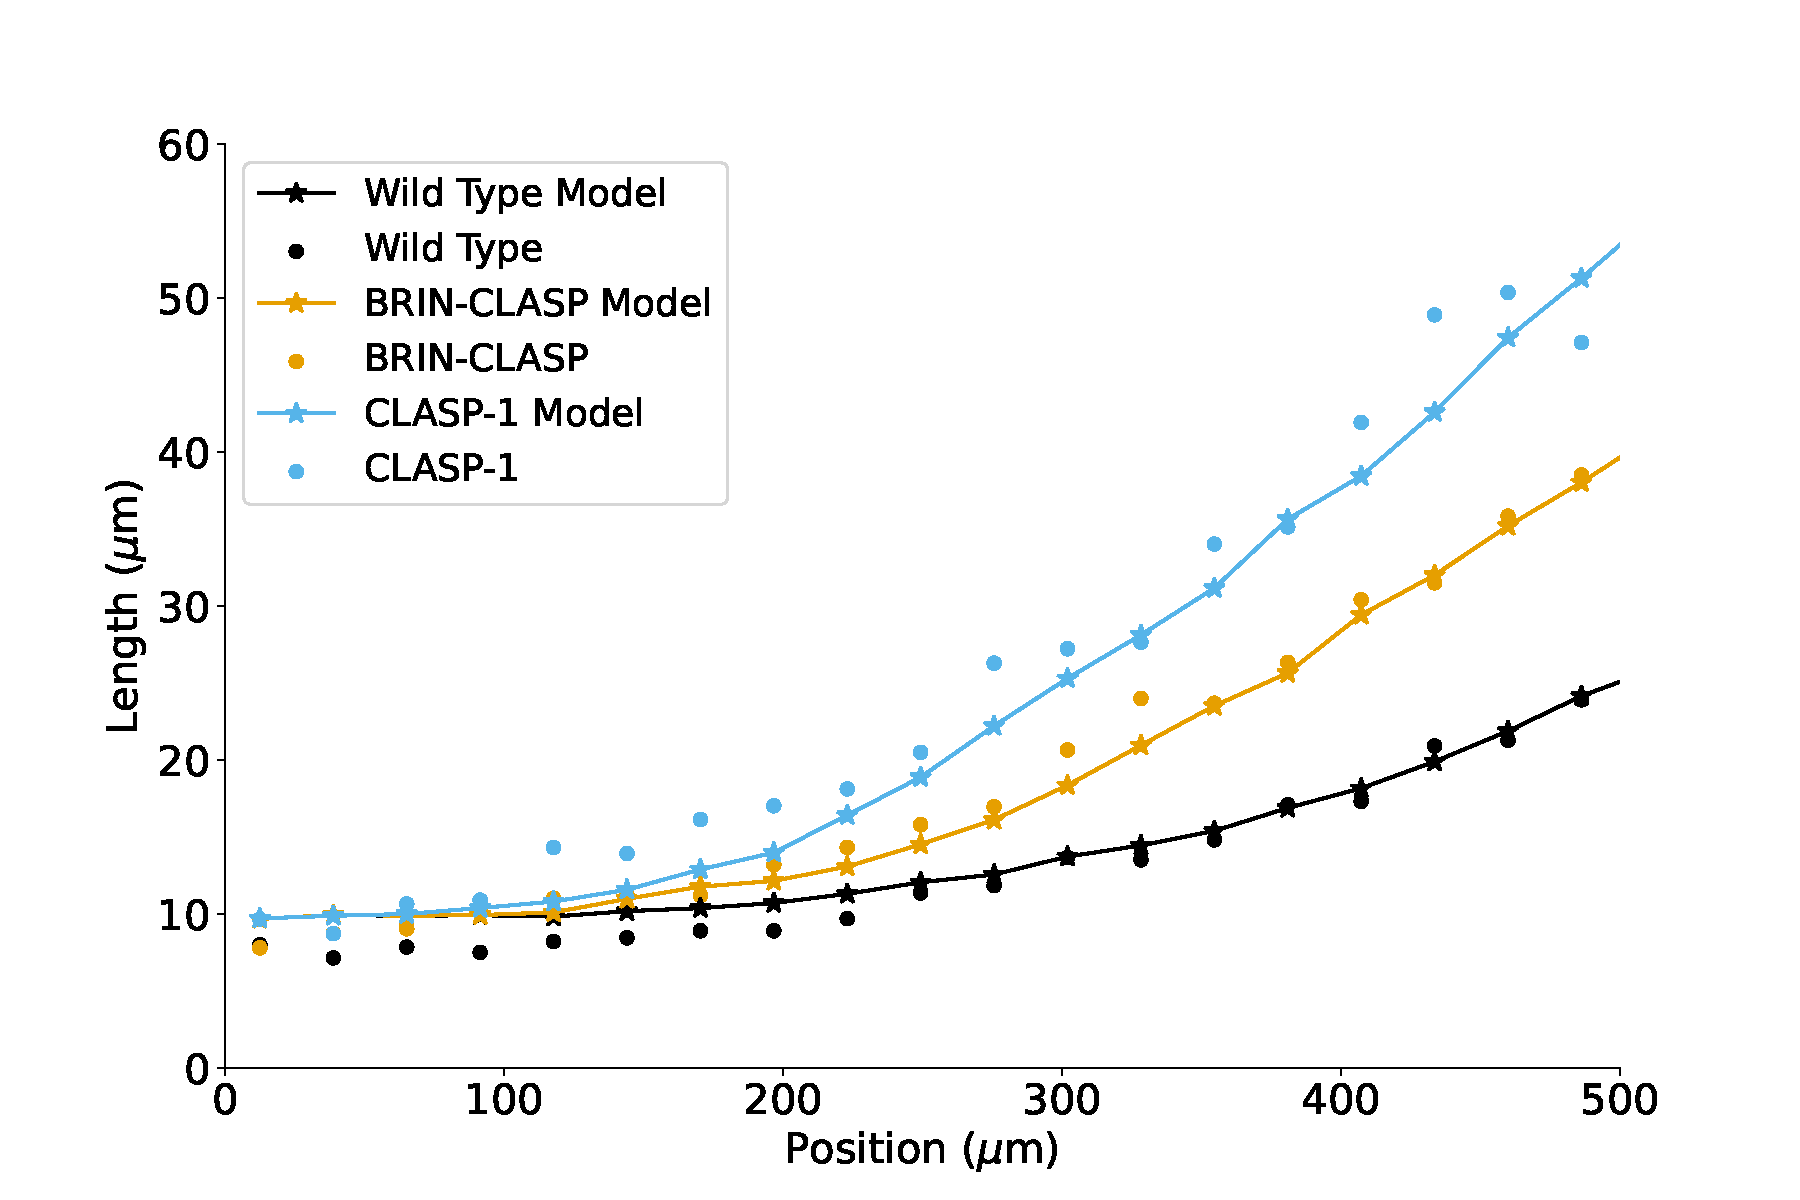
\includegraphics[width=\textwidth]{column-modified-fit.pdf}
  \caption{Model results after modifying CLASP's influence on division.
  By reversing the effect of CLASP on cell division at high concentrations, the RMSE of the model decreased from $10.401$ to $5.630$.
Under the new model, mean cell lengths in the wild type and \emph{brinCLASPpro} mutants are clearly differentiated. }
  \label{column-modified-fit}
\end{figure}

 
\section*{Discussion}\label{sec12}

In this paper, we developed a novel ODE model of BR/CLASP signalling in the meristem of \emph{A. thaliana} roots.
This model was informed by \emph{in-vivo} experiments involving the CLASP protein \cite{ambrose2011, ruan2018, halat2022} and previous models of the BRI1 receptor system \cite{vanesse2012}.
We also incorporated multiple supplementary results \cite{wang2001, cano-delgado2004} to determine appropriate ranges for our parameter values.
Initially, our model could not differentiate the \emph{brinCLASPpro} mutant from the wild type.
However, modifying our model so that cell division is inhibited by superphysiological concentrations of CLASP was sufficient to recover the \emph{brinCLASPpro} mutant.
We believe the biological mechanism driving this behaviour is related to the role of the CLASP protein in ensuring microtubule stability during each phase of the cell cycle.
Under our hypothesis, high concentrations of CLASP prevent the TFBs that form during interphase from disassembling during mitosis, leading to a slower cell cycle.
However, further experimental research is needed to confirm this result.

Our model makes use of two ``sizer'' mechanisms for determining cell state.
The sizer mechanism for cell differentiation proposed by Pavelescu et al., 2016 \cite{pavelescu2016} yields a model where root length depends solely on the number of division events, since all cells eventually reach the same size.
While this modelling assumption appears to be reasonable for the wild type, it could break down in mutants with an unusually low or high division rate. 
The second sizer mechanism governs exit from the division zone by placing a soft upper bound on the length of a mitotic cell.
This mechanism was necessary to prevent the number of cells from growing exponentially in our model.
However, other mechanisms for restricting cell division involving cell age (``timer''), cell position (``ruler''), or BES1 signalling could also perform the same function.
Further modelling research exploring alternatives to these sizer mechanisms would help elucidate the true processes underlying cell elongation and cell division.
 
Multiple simplifying assumptions were made to reduce the dimensionality of the parameter space and prevent overfitting.
In particular, our model assumed that the BL concentration function $B(z)$ remained unchanged under the two mutations.
Since our intracellular signalling model suggested that BES1 signalling and thus cell elongation was primarily determined by BL and not BRI1, this is a strong assumption.
While we are unaware of any signalling pathways involving CLASP that would cause a change in the BL concentration between the wild type, \emph{brinCLASPpro}, and \emph{clasp-1} mutants, it is possible that such a pathway exists.
If BL is indeed coupled with CLASP, this interaction could be responsible for the differences in cell lengths between the different genotypes.
Furthermore, our model of cell elongation abstracted away a complex signalling network involving wall-loosening enzymes, cellulose microfibrils, and microtubules \cite{smithers2024}.
Considering the mechanics of the cell wall would improve parameter estimation in subsequent models and provide more accurate information about the influence of BES1 signalling on cell elongation.
Finally, our model of cell division omits the stages of the cell cycle, such as the formation of the mitotic spindle.
A more intricate model of cell state would give us a better understanding of how the CLASP protein affects cell division, which could either verify or disprove our conclusions.

% TODO: Cite others -- who?

Further modelling work in this area would benefit from ``zooming in'' on cell-scale phenomena and ``zooming out'' to incorporate CLASP in other models of the root apical meristem.
There have been multiple efforts in recent years to simulate the formation of microtubules on the lipid membrane \cite{tian2023, tindemans2014, allard2010a}.
These models have given us a better understanding of how microtubules behave in the presence of the CLASP protein.
By coarse-graining the key results from these models, we can develop a better understanding of how microtubules influence both cell and organ development.
There have also been many efforts to model the auxin signalling network \cite{grieneisen2007, dimambro2017}.
These models have improved our understanding of hormone fluxes across the entire root, including between cell columns.
Comprehensive models of the \emph{A. thaliana} root have included many molecules in addition to auxin, including cytokinins \cite{salvi2020}, ethylene \cite{moore2024}, and gibberelin \cite{muraro2016}.
We believe that the BR/CLASP signalling network should also be included in these models, as CLASP has already been shown to influence the recycling of PIN2 auxin transporters in the root apical meristem \cite{ambrose2013}.
Developing models of how intracellular signalling drives cell and organ development in roots remains a pressing area for further research.
By using models to engineer resilient plant genotypes, we can protect our crops from droughts, heat waves, and other adverse events.

\backmatter

\bmhead*{Supplementary Information}

The code for this project is available on \href{https://github.com/rileywheadon/clasp-model}{Github}.

\bmhead*{Acknowledgements}

TBD

\section*{Declarations}

TBD

\bibliography{sources}

\begin{appendices}

\section{Data Collection and Preparation}\label{secA1}

Five distinct lines of \emph{A. thaliana} were grown in the lab.
Table \ref{plant-lines} contains the number of plants in each line.
The wild type line consists of \emph{A. thaliana} plants that have not been modified in any way.
All four remaining lines have the \emph{clasp-1} mutation, which prevents transcription of the CLASP protein \cite{ambrose2007}.
In three of the lines with the \emph{clasp-1} mutation, functional replacement of CLASP is achieved through the \emph{CLASPpro:GFP-CLASP} or \emph{brinCLASPpro:GFP-CLASP} mutations \cite{ambrose2007, ruan2018}.
The introduction of \emph{GFP-CLASP} (green fluorescent protein CLASP) makes it possible to estimate \emph{in-vivo} CLASP concentrations using fluorescence microscopy \cite{ambrose2007, ruan2018}.
Therefore, the \emph{CLASPpro:GFP-CLASP/clasp-1} and wild type lines have equivalent phenotypes.
The \emph{brinCLASPpro:GFP-CLASP/clasp-1} lines 3 and 15 will be considered together as the \emph{brinCLASPpro} mutant for the sake of brevity.
A plot of the cell surface area and cell number data collected from all five lines is shown in Figure \ref{data-unprocesed}.

\begin{table}[!ht]
\centering
\caption{Number of \emph{A. thaliana} roots analyzed in each genetic line.}
\label{plant-lines}
\begin{tabular}{@{}lll@{}}
\toprule
Line & \# Plants \\
\midrule
\emph{Wild Type}  & 11  \\
\emph{CLASPpro:GFP-CLASP/clasp-1} & 18 \\
\emph{brinCLASPpro:GFP-CLASP/clasp-1} (3) & 17 \\
\emph{brinCLASPpro:GFP-CLASP/clasp-1} (15) & 11 \\
\emph{clasp-1} & 20 \\
\botrule
\end{tabular}
\end{table}

\begin{figure}
  \centering
  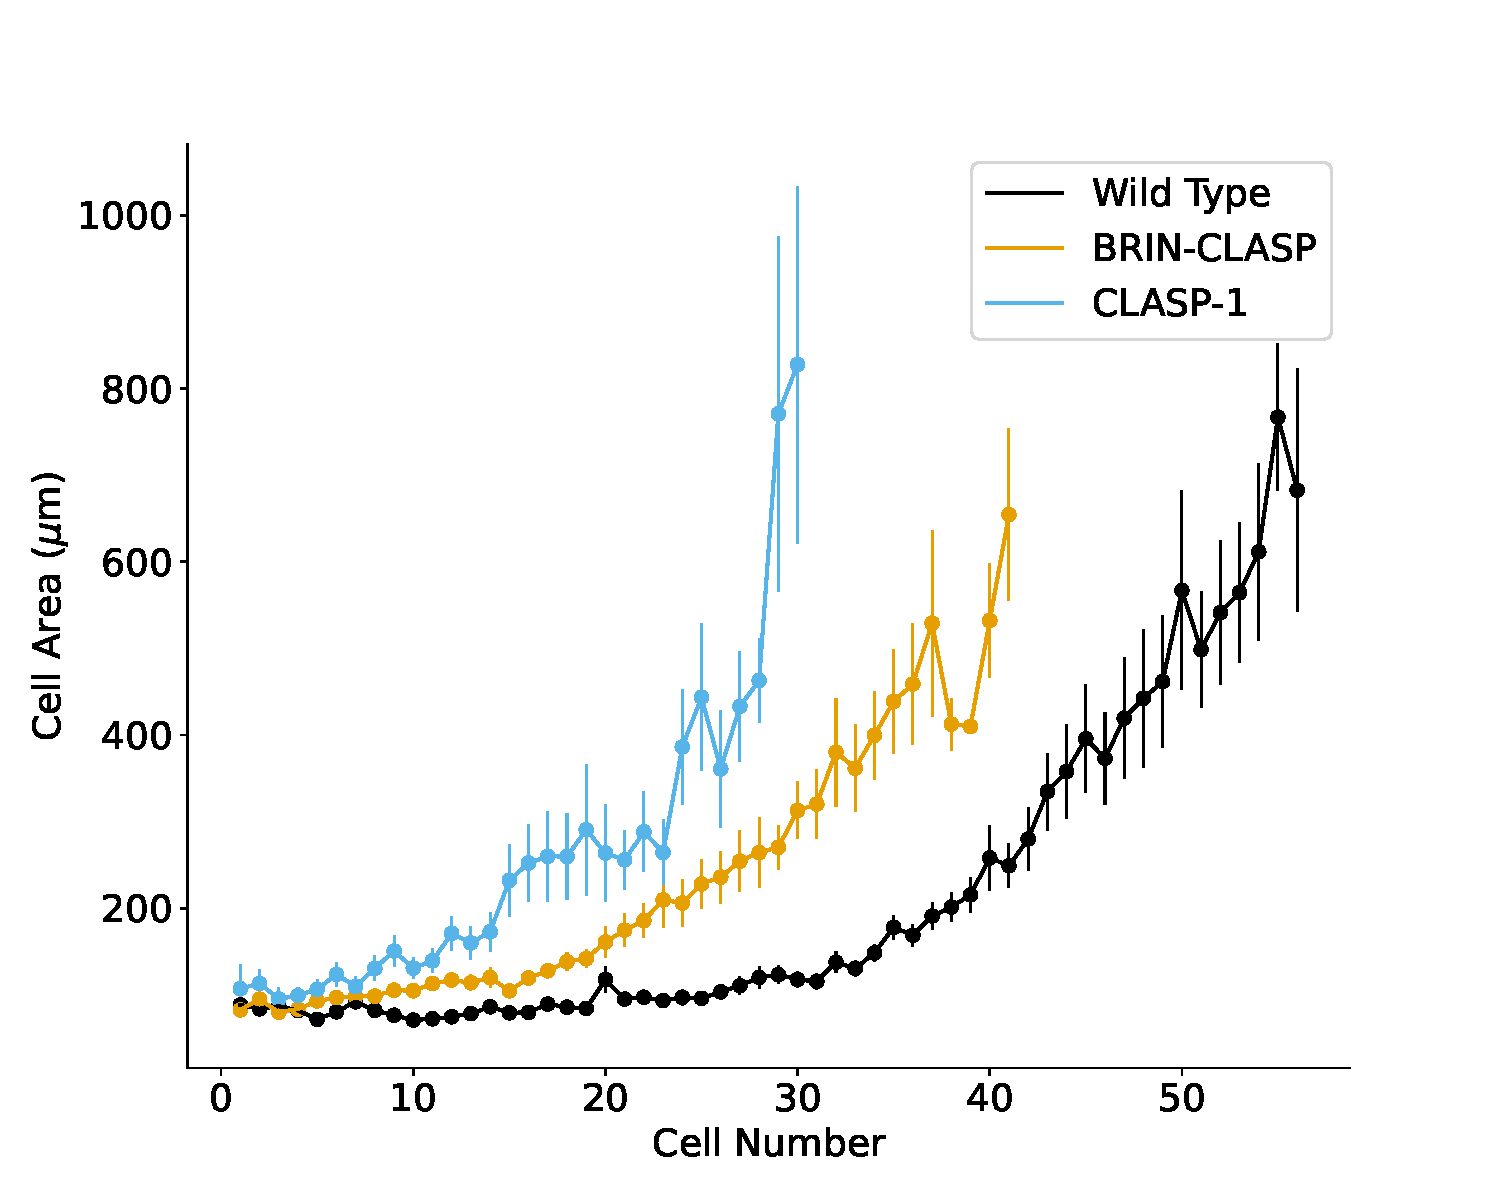
\includegraphics[width=\textwidth]{data-unprocessed.pdf}
  \caption{Raw data from the five distinct lines of \emph{A. thaliana} grown for this paper.
  The ``Wild Type'' data shown in black comes from both the \emph{Wild Type} and \emph{CLASPpro:GFP-CLASP/clasp-1} lines.
The ``BRIN-CLASP'' data shown in orange comes from the \emph{brinCLASPpro:GFP-CLASP/clasp-1} lines (3) and (15).
The ``CLASP-1'' data comes entirely from the \emph{clasp-1} lines.
Differences in cell area between the mutants exhibit clear statistical significance. }
  \label{data-unprocesed}
\end{figure}

The raw data in units of cell number and cell area were transformed into units of cell position and cell length via the following procedure.
First, the vertical cell faces were assumed to be flat so that the cross-sectional areas observed in the microscopy images correspond exactly to the length of the cell multiplied by its radius.
Then, the position of each cell was determined by taking the cumulative sum of the lengths of the cells underneath it.
By convention, cell position is relative to the quiescent centre, so proximal cells are located ``higher''.
Missing data in the division zone was imputed using the average cell length by cell number.
The resulting dataset contained position-length pairs from $0\um$ to $1500\um$ above the quiescent centre.
However, the data above $500\um$ was omitted from subsequent analyses since it was noisy and sparse. 

\begin{figure}
  \centering
  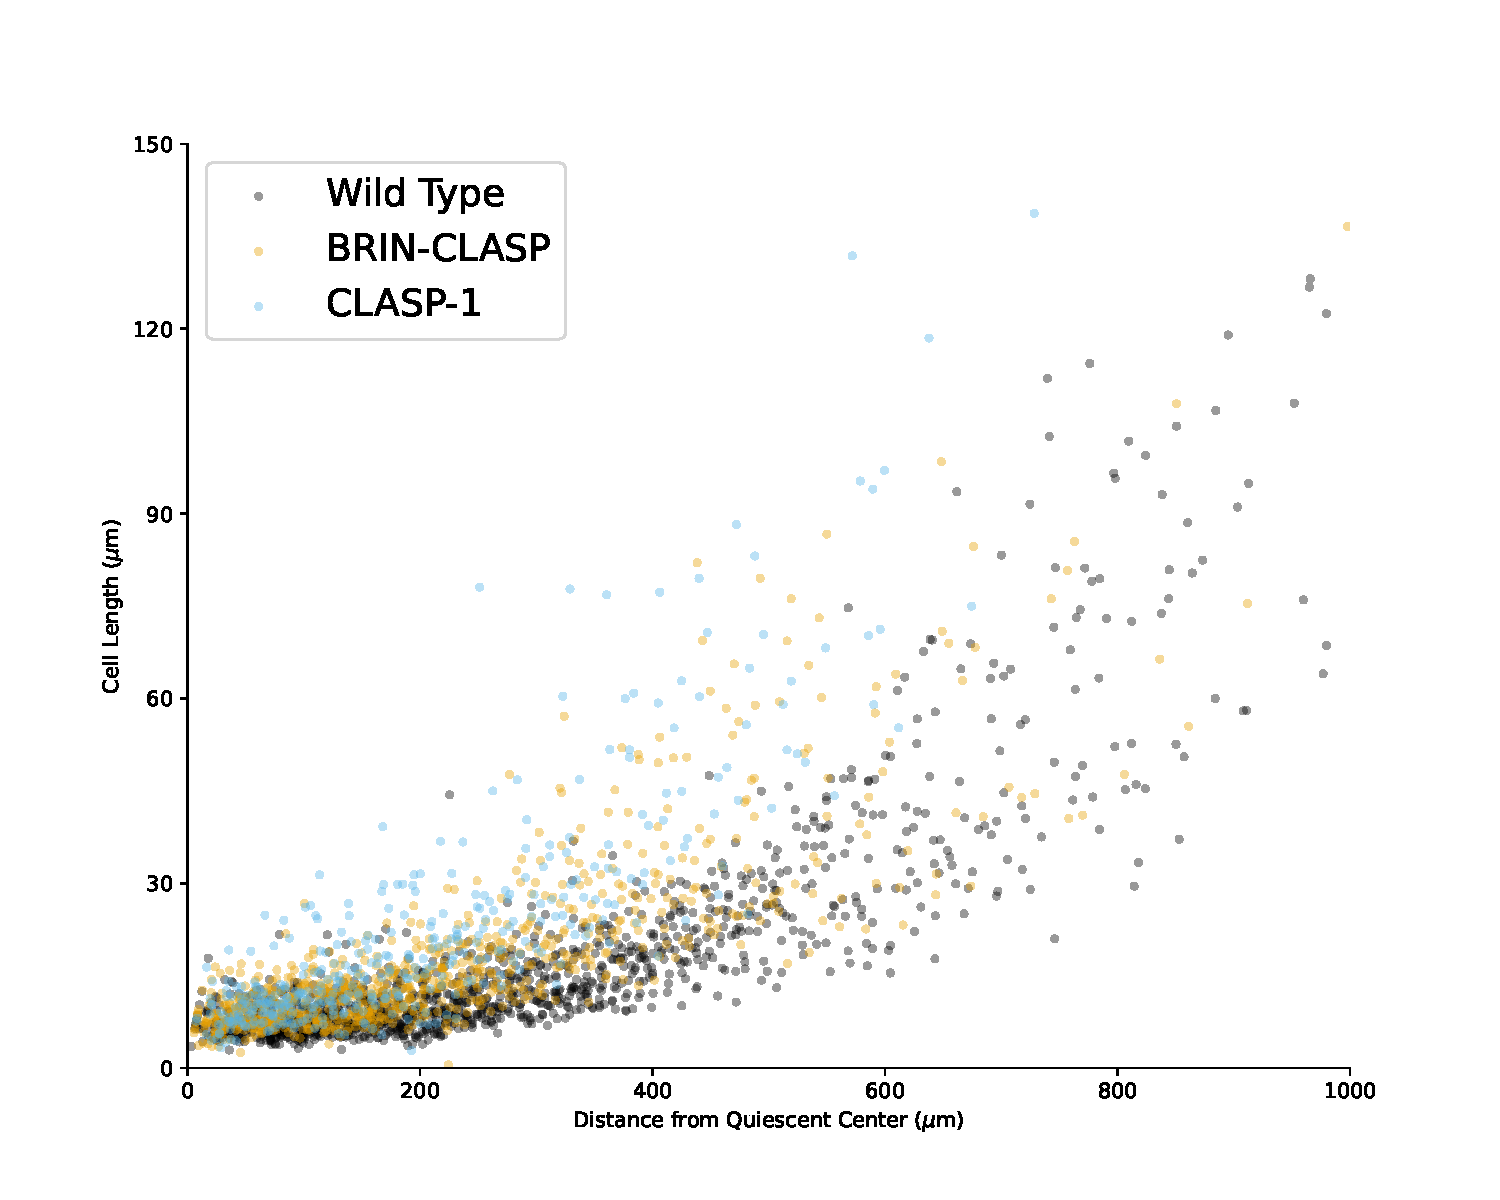
\includegraphics[width=\textwidth]{data-trichoblast.pdf}
  \caption{Raw data collected from trichoblast cells in \emph{A. thaliana}.
  There is a high density of data points in the distal region of the meristem ($< 500\um$), but significantly fewer data points between $500\um$ and $1000\um$, especially in the \emph{brinCLASPpro} and \emph{clasp-1} mutants.
After binning this data (not shown) and computing the standard errors, we found that the data above $500\um$ was too noisy to differentiate the wild type and \emph{brinCLASPpro} mutant. }
  \label{data}
\end{figure}

\section{Model Derivation}\label{secA2}

We begin with the mass balance equations \eqref{eq} for the BRI1 receptor system proposed by van Esse et al., 2012 \cite{vanesse2012}.

\begin{equation}
\begin{cases}
    \label{eq}
    R_{B} = \dfrac{R_{F} \cdot B_{F}}{K_{d}} \\
    R_{T} = R_{B} + R_{F} \\
    B(z) = B_{B} + B_{F} 
\end{cases}
\end{equation}

In Equation \ref{eq}, $R_{T}$, $R_{F}$, and $R_{B}$ denote the concentrations of total BRI1 receptors, free BRI1 receptors, and bound BRI1 receptors respectively.
$B(z)$ is the BL concentration as an increasing function of cell position.
Additionally, $B_{F}$ and $B_{B}$ are the concentration of free and bound BL ligand respectively.
$K_{d}$ is the dissociation rate.
By rearranging Equation \ref{eq}, we can solve for $R_{B}$ as a function of $R_{T}$ and $B(z)$ as shown in Equation \ref{bri1}.

\begin{equation}
\label{bri1}
R_{B}(z) = \frac{(B + R_{T} + K_{d}) - \sqrt{(B + R_{T} + K_{d})^{2} - 4 \cdot  R_{T} \cdot B}}{2}
\end{equation}

Using the function for $R_{B}$ shown in Equation \ref{bri1} we can derive a model of the intracellular dynamics of the BR/CLASP signalling network over time using the system of ordinary differential equations (ODEs) shown in Equation \ref{intracellular-ode}.

\begin{equation}
\label{intracellular-ode}
\begin{aligned}
  \frac{ dS }{ dt } &= s_{0}R_{B}(z) - s_{1} S \\[5pt]
  \frac{ dC }{ dt } &= (c_{0} - c_{2}S) - c_{1}C \\[5pt]
  \frac{ dR_{T} }{ dt } &= (r_{0}  + r_{2}C) - r_{1}R_{T}
\end{aligned}
\end{equation}

The parameters $s_{0}$, $c_{0}$, and $r_{0}$ represent basal production rates for the BES1 transcription factor $S$, CLASP $C$, and total BRI1 receptors $R_{T}$ respectively.
The parameters $s_{1}$, $c_{1}$, and $r_{1}$ represent decay rates for the same molecules.
The parameter $c_{2}$ represents the rate at which the BES1 transcription factor inhibits the CLASP promoter while $r_{2}$ represents the rate at which CLASP promotes the recycling of endocytosed BRI1 receptors.
Next, we assume that intracellular levels of BES1, CLASP, and BRI1 are in quasi-steady state (QSS), which means that $\frac{dS}{dt} = \frac{dC}{dt} = \frac{dR_{T}}{dt} = 0$.
The QSS assumption gives us explicit formulas for $S$, $C$, and $R_{T}$ in terms of $R_{B}$ as shown in Equation \ref{intracellular-qss}. 

\begin{equation}
\label{intracellular-qss}
\begin{aligned}
  S(z) &= \frac{ s_{0} R_{B}(z)}{ s_{1} } \\[5pt]
  C(z) &= \frac{ c_{0} - c_{2}S }{ c_{1} } \\[5pt]
  R_{T}(z) &=\frac{ r_{0} + r_{2}C }{r_{1} } 
\end{aligned}
\end{equation}

Since the BES1 transcription factor $S$ is just a scalar multiple of $R_{B}$ under the QSS assumption, we will use $R_{B}$ in place of $S$ and rescale $c_{2}$ accordingly.
It is known from \emph{in-vivo} experiments \cite{ruan2018} that the total concentration of BRI1 receptors in the \emph{clasp-1} mutant is approximately $65\%$ of the concentration in the wild type.
Since the wild type root has an average BRI1 receptor concentration of approximately $62\nm$ \cite{vanesse2012}, the \emph{clasp-1} mutant should have a BRI1 receptor concentration of roughly $(62 \cdot 0.65)\nm$.
If we nondimensionalize Equation \ref{intracellular-qss} such that $C = 1$ is the average CLASP concentration in the wild type and recall that $C = 0$ in the \emph{clasp-1} mutant, we can determine $r_{2} / r_{1}$ as shown in Equation \ref{clasp-simplified}.

\begin{equation}
\label{clasp-simplified}
\left.\begin{aligned}
  62 = (r_{0} + r_{2}) / r_{1} \\
  (62 \cdot 0.65) = r_{0} / r_{1}
\end{aligned}\right\rbrace \Rightarrow  \frac{r_{2}}{r_{1}} = (62 \cdot 0.35)
\end{equation}

Then, we define the new parameters $\beta_{0} = \frac{c_{0}}{c_{1}}$, $\beta_{1} = \frac{c_{2}s_{0}}{c_{1}s_{1}}$.
This gives us a simplified system of equations \eqref{clasp-rt-final} for the intracellular protein concentrations of CLASP and BRI1 under the QSS assumption and after nondimensionalization.

\begin{equation}
\label{clasp-rt-final}
\begin{aligned}
  C(z) &= \beta_{0} - \beta_{1}R_{B}(z) \\[5pt]
  R_{T}(z) &= 62 (0.65 + 0.35 C)
\end{aligned}
\end{equation}

Producing this derivation required multiple estimates of biological constants from the literature.
Experimental results were also used to choose reasonable ranges for parameter fitting.
A complete list of the sources used in our intracellular signalling model is provided in Table \ref{parameter-values}.
For the fitting of the intracellular signalling model we allowed $K_{d}$ to vary between $7\nm$ and $55\nm$.

\begin{table}[!ht]
\centering
\caption{Parameter estimates used in the intracellular signalling model.} 
\label{parameter-values}
\begin{tabular}{@{}lll@{}}
\toprule
Parameter & Estimate & Source \\ 
\midrule
$R_{T}$ & $62\nm$ & van Esse et al., 2012 \cite{vanesse2012} \\
$K_{d}$ & $7.4-15\nm$ & Wang et al., 2001 \cite{wang2001} \\
$K_{d}$ & $55\nm$ & Ca\~no-Delgado et al., 2004 \cite{cano-delgado2004} \\
$B$ & $<1 \nm$ & van Esse et al., 2012 \cite{vanesse2012} \\
\botrule
\end{tabular}
\end{table}

\section{Atrichoblast Model}\label{secA4}

The data used in this project was collected from trichoblast and atrichoblast cells from the epidermal cell columns of \emph{A. thaliana} roots.
In this appendix, we contrast the fitted models for both of these datasets.
Figure \ref{column-atrichoblast-fit} presents the fitted model for atrichoblast cells, while Table \ref{column-atrichoblast-parameters} compares parameter values for the trichoblast and atrichoblast cell column models.

\begin{figure}[!htp]
  \centering
  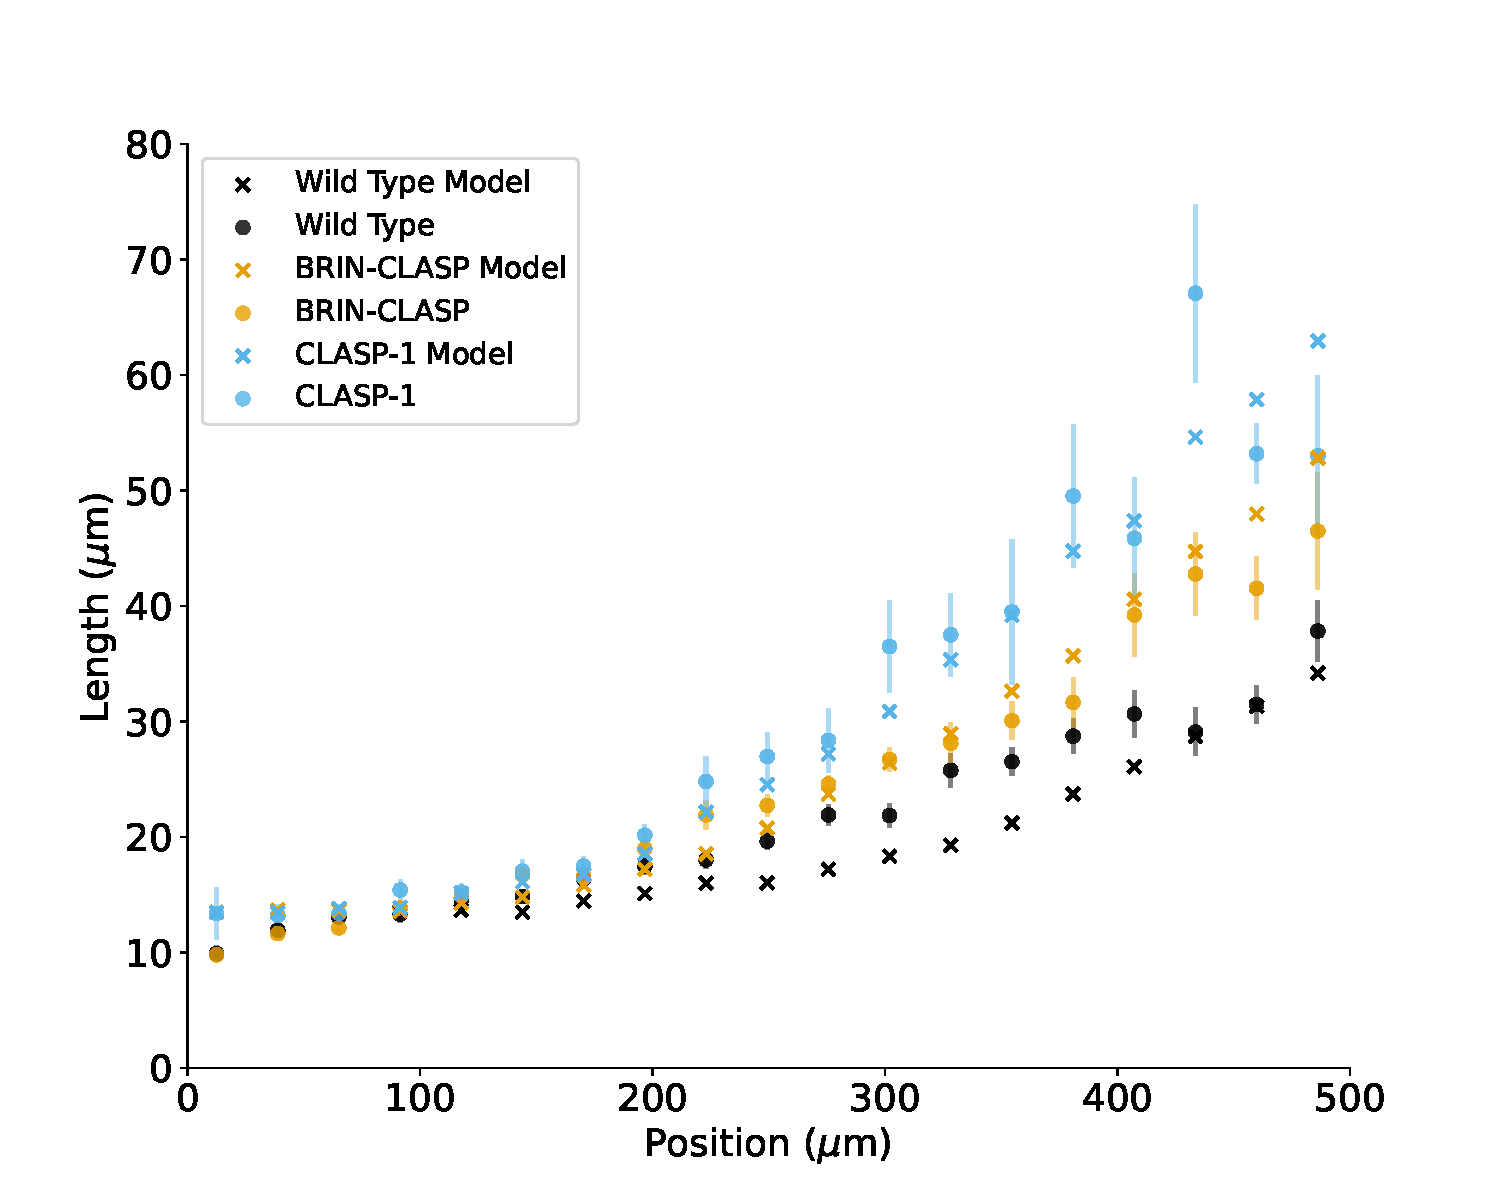
\includegraphics[width=\textwidth]{column-atrichoblast-fit.pdf}
  \caption{Results of fitting the model to atrichoblast data.
    The fitted model underestimates wild type cell length between $200\um$ and $300\um$ but captures the general differences between the three genotypes.
Compared to trichoblast cells, atrichoblast cells exhibit less differentiation between the mutants and have longer cells on average. }
  \label{column-atrichoblast-fit}
\end{figure}

\begin{table}[!htp]
\centering
\caption{Optimal parameter values for the atrichoblast cell column model compared to the trichoblast cell column model.
Both models use the biphasic CLASP function described in the paper.
The atrichoblast model has higher $m$ and $\delta_{0}$ parameters, which makes sense because atrichoblast cells are larger.
Other parameters remained roughly the same, which suggests that the estimated parameters are relatively robust to changes in the data.} 
\label{column-atrichoblast-parameters}
\begin{tabular}{@{}lllllllll@{}}
\toprule
Model & RMSE & $m$ & $\gamma_{0}$ & $\gamma_{1}$ & $\delta_{0}$ & $\delta_{1}$ & $\delta_{2}$ \\
\midrule
Trichoblast & $5.630$ & $14.32$ & $0.500$ & $4.148$ & $20.26$ & $1.870$ & $1.278$ \\
Atrichoblast & $10.51$ & $19.70$ & $0.487$ & $4.148$ & $27.50$ & $1.932$ & $1.333$ \\
\botrule
\end{tabular}
\end{table}

\section{Additional Figures}\label{secA3}

Figure \ref{column-original-profile} and Figure \ref{column-original-histogram} contain more information about the original cell column model, which failed to differentiate between the wild type and \emph{brinCLASPpro} mutant.
In particular, these figures show that the distribution of cell division positions and thus the size of the division zone is nearly identical in the wild type and \emph{brinCLASPpro} mutant under our initial model. 
Figure \ref{column-modified-profile} and Figure \ref{column-modified-histogram} contain the same visualizations as Figures \ref{column-original-profile} and \ref{column-original-histogram} for the modified cell column model.
These figures provide further evidence that modifying the division equation to introduce a local maximum at an intermediate concentration of CLASP is sufficient to differentiate the wild type and \emph{brinCLASPpro} mutant.
Additionally, these figures makes quantitative estimates for the size of the division zone in all three genotypes.

\begin{figure}[!htp]
  \centering
  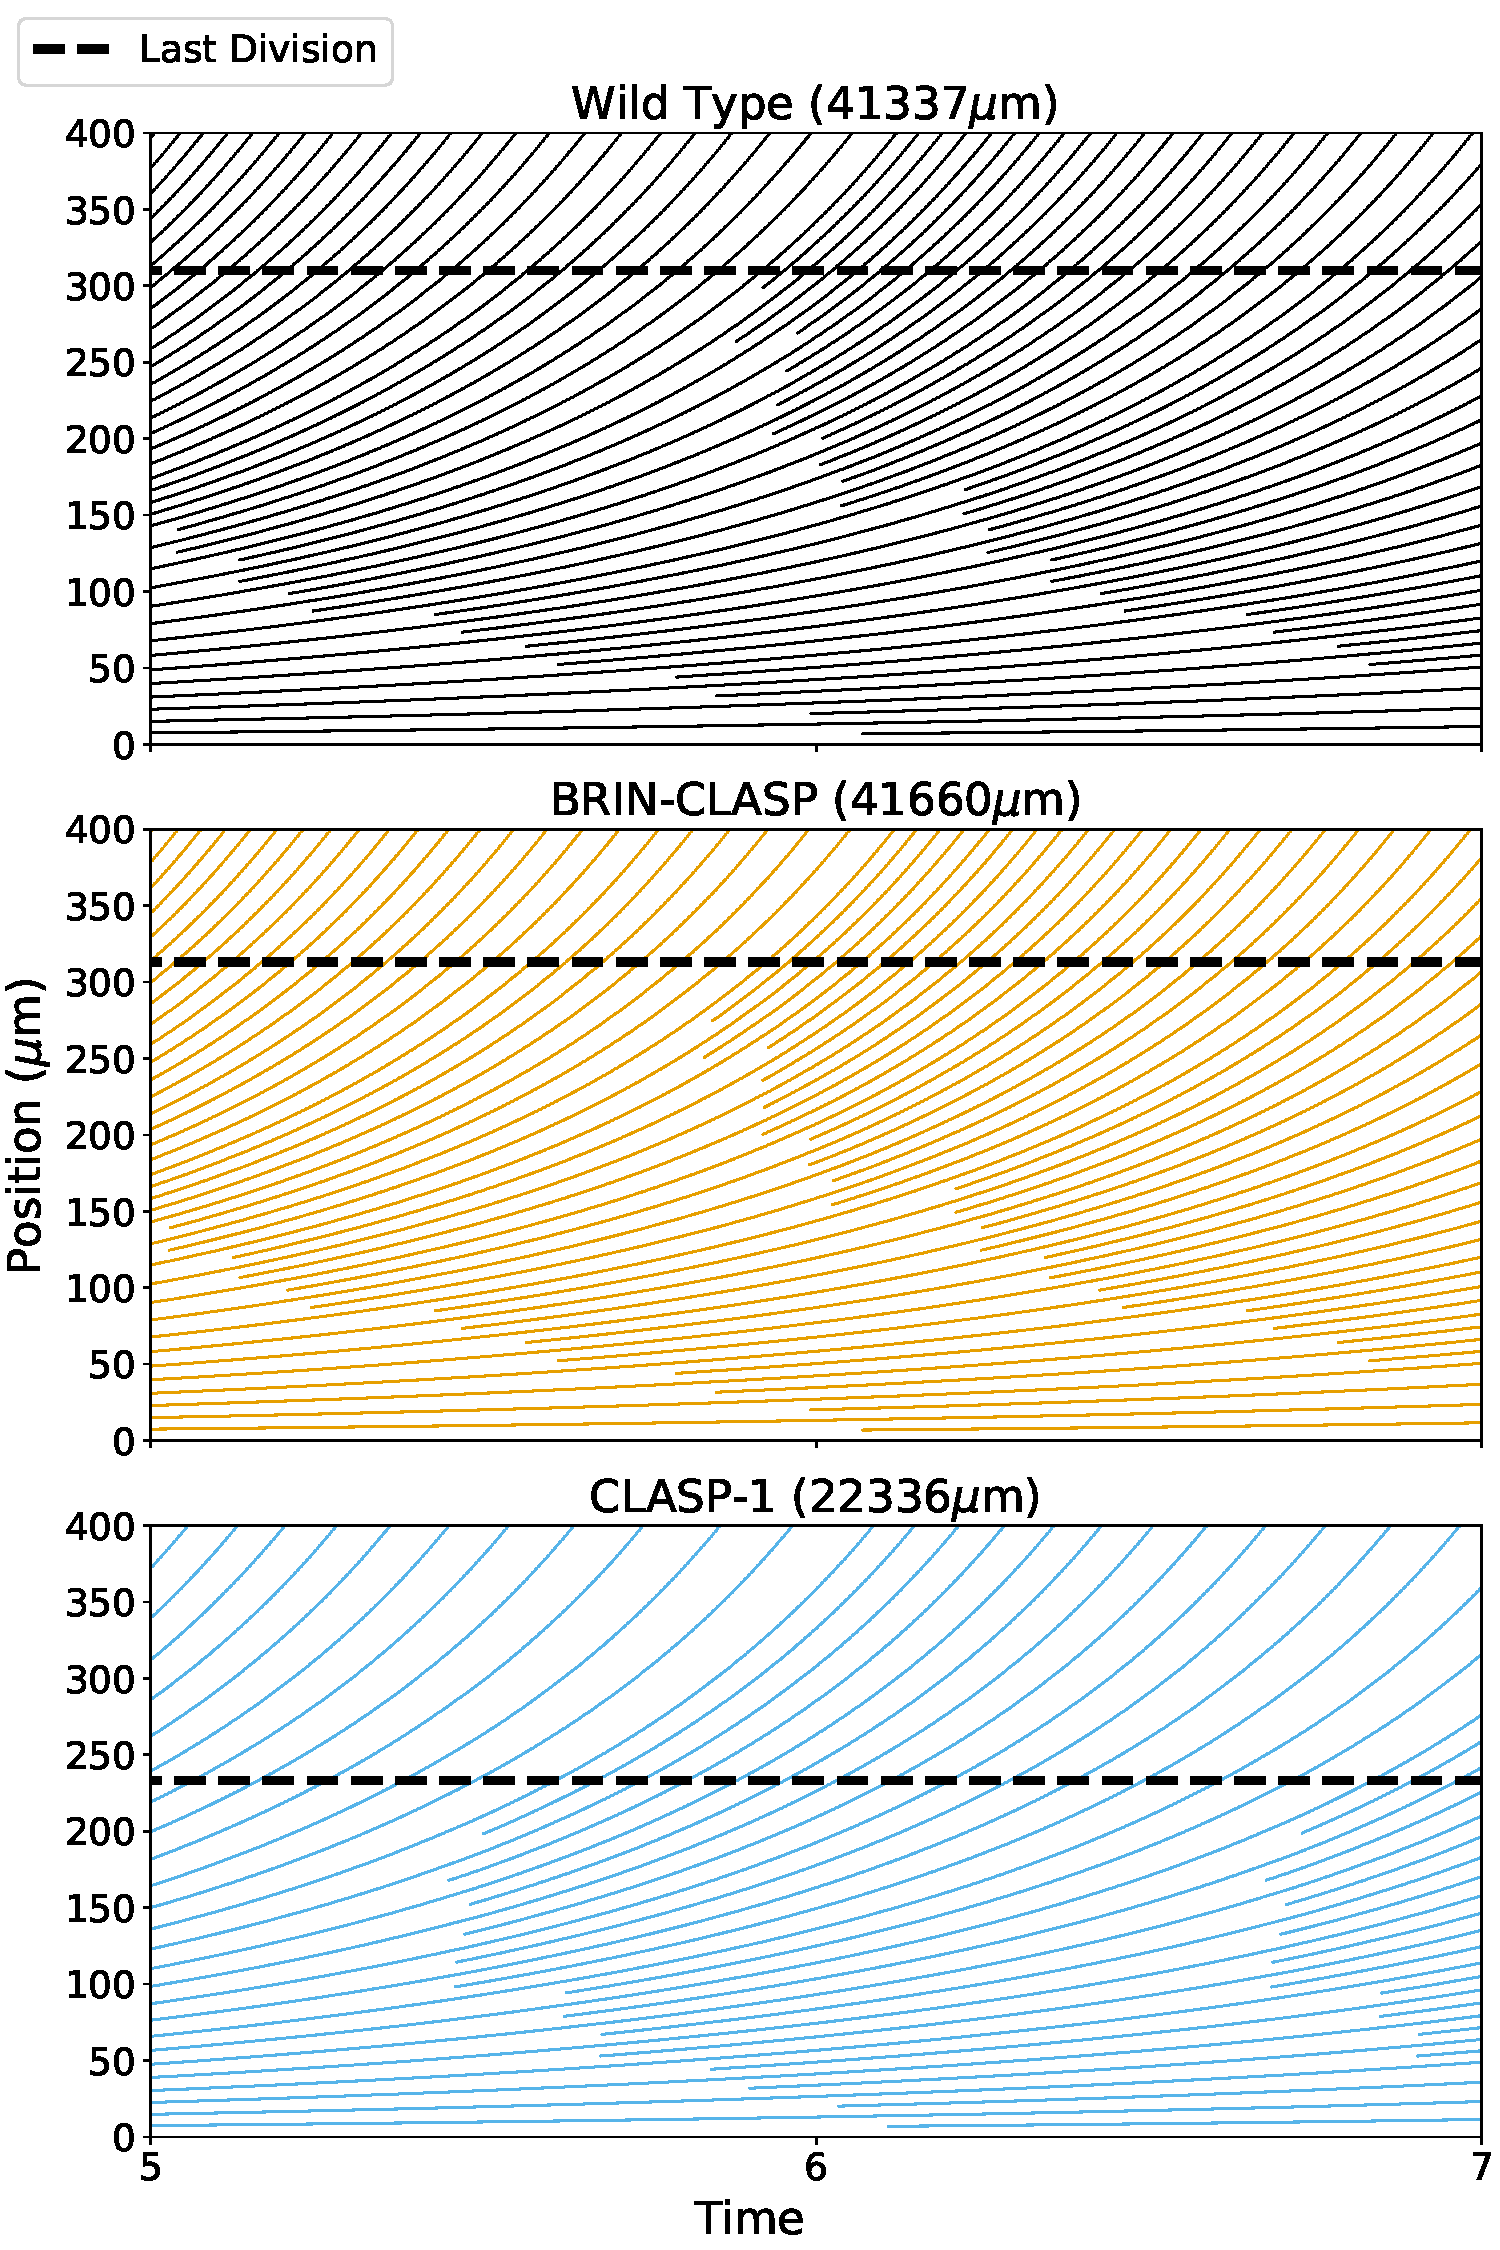
\includegraphics[height=480pt]{column-original-profile.pdf}
  \caption{Cell column projection for the original cell column model. The $x$-axis represents a (dimensionless) time variable while the $y$-axis represents distance from the quiescent centre in $\um$. The dotted black line is the highest position at which a division event occurred over the entire simulation. This point can be interpreted as the height of the division zone. Both the wild type and the \emph{brinCLASPpro} roots have a division zone that is roughly $300\um$ long, while the \emph{clasp-1} mutant has a shorter division zone at approximately $230\um$.}
  \label{column-original-profile}
\end{figure}

\begin{figure}[!htp]
  \centering
  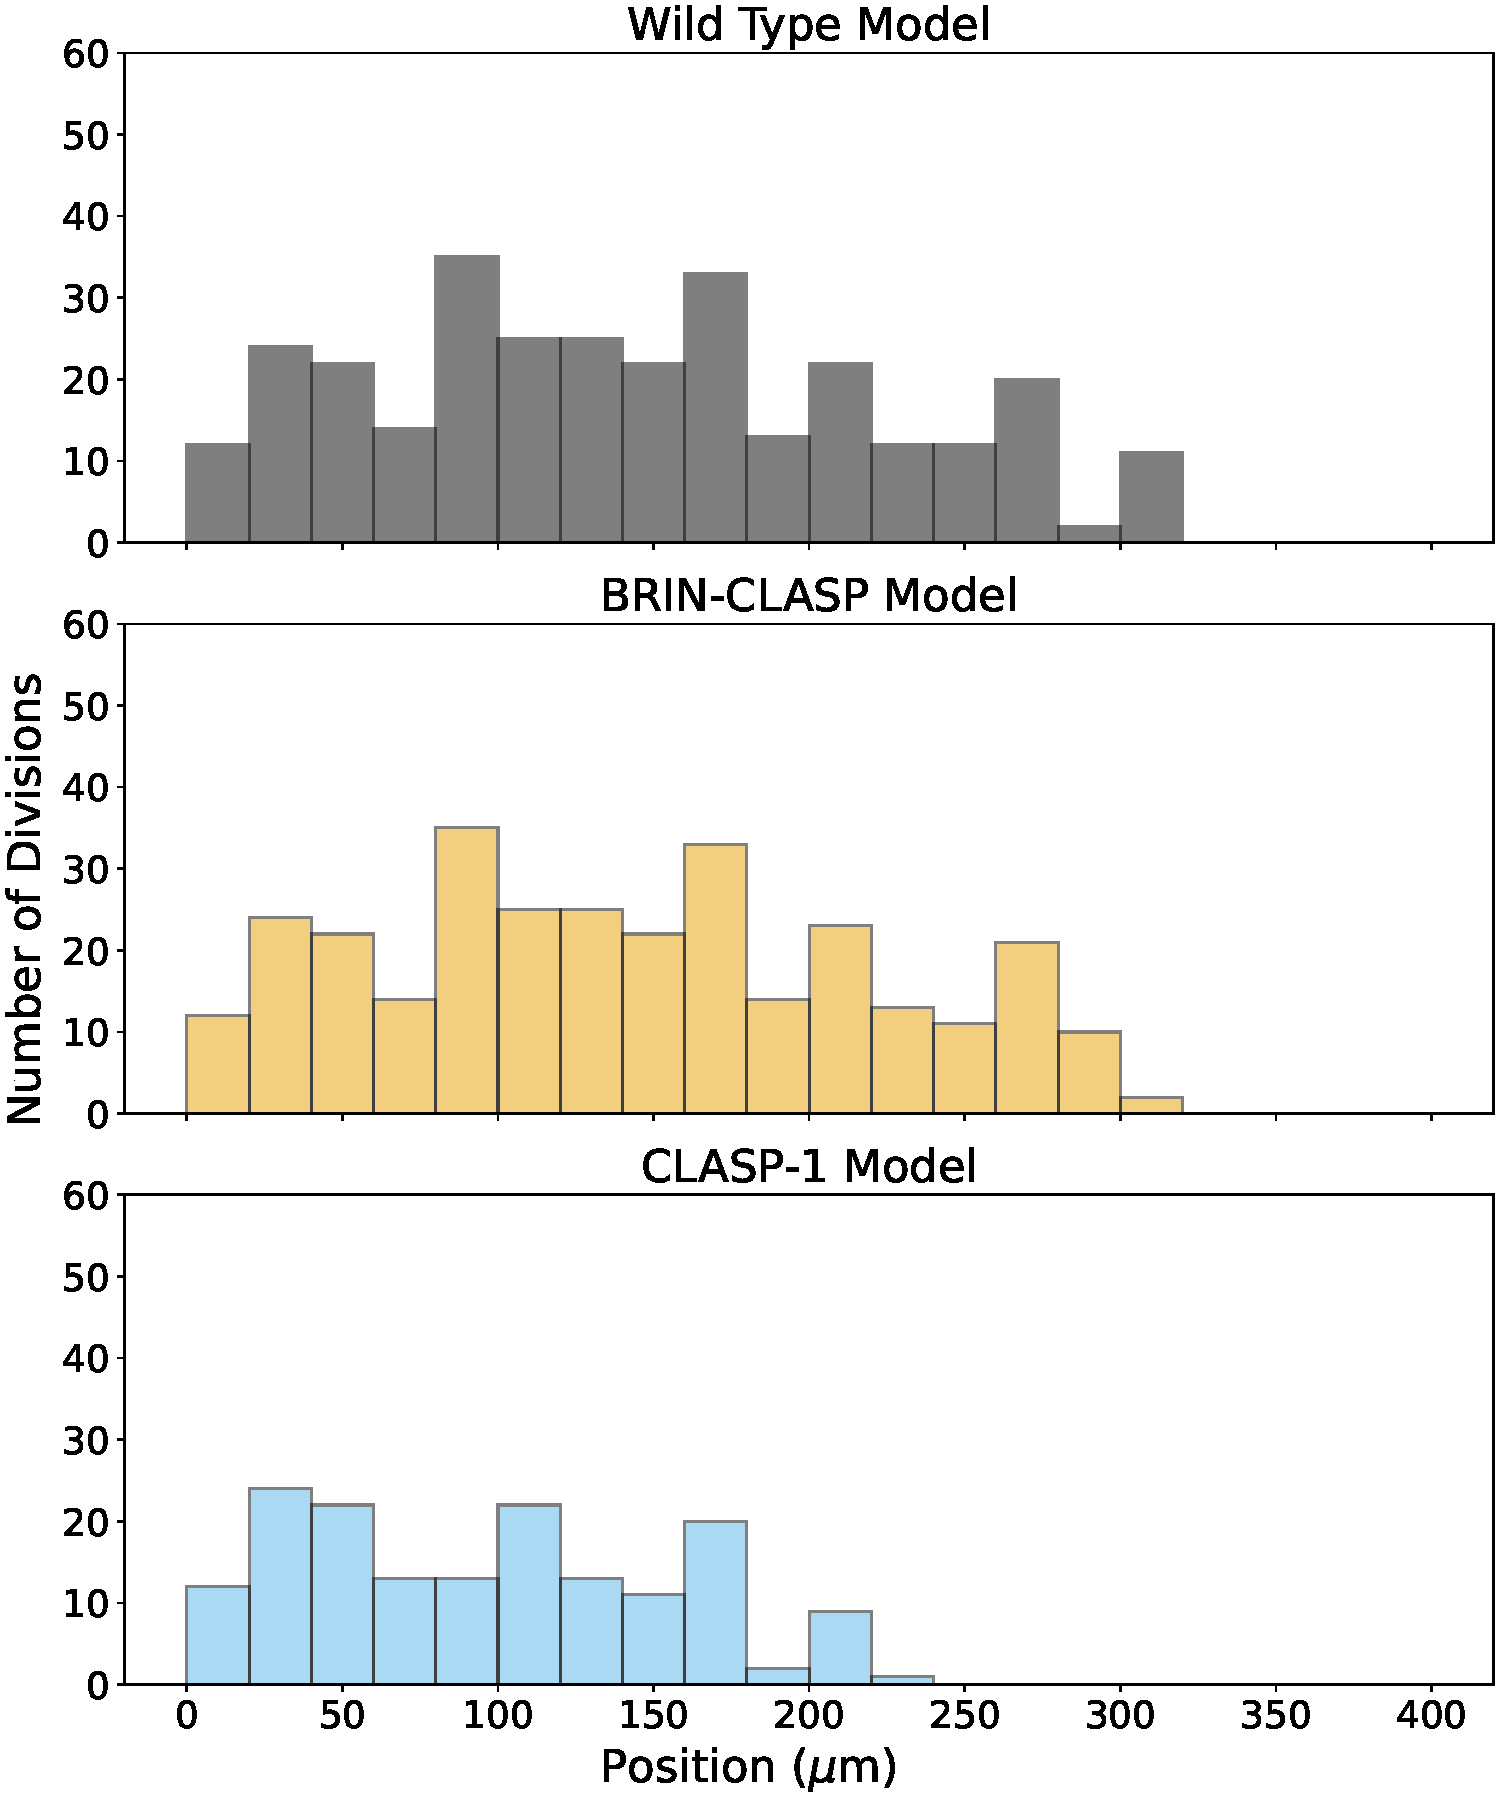
\includegraphics[width=\textwidth]{column-original-histogram.pdf}
  \caption{Histogram of division by cell position for the original cell column model. As in all previous figures, cell position is measured as distance from the quiescent centre in $\um$. The division locations have a unimodal distribution for all three genotypes, with some noise between the bins. The distribution of division locations is nearly identical for the \emph{brinCLASPpro} mutant and wild type roots, which reflects the failure of this model to clearly differentiate these two genotypes.}
  \label{column-original-histogram}
\end{figure}

\begin{figure}[!htp]
  \centering
  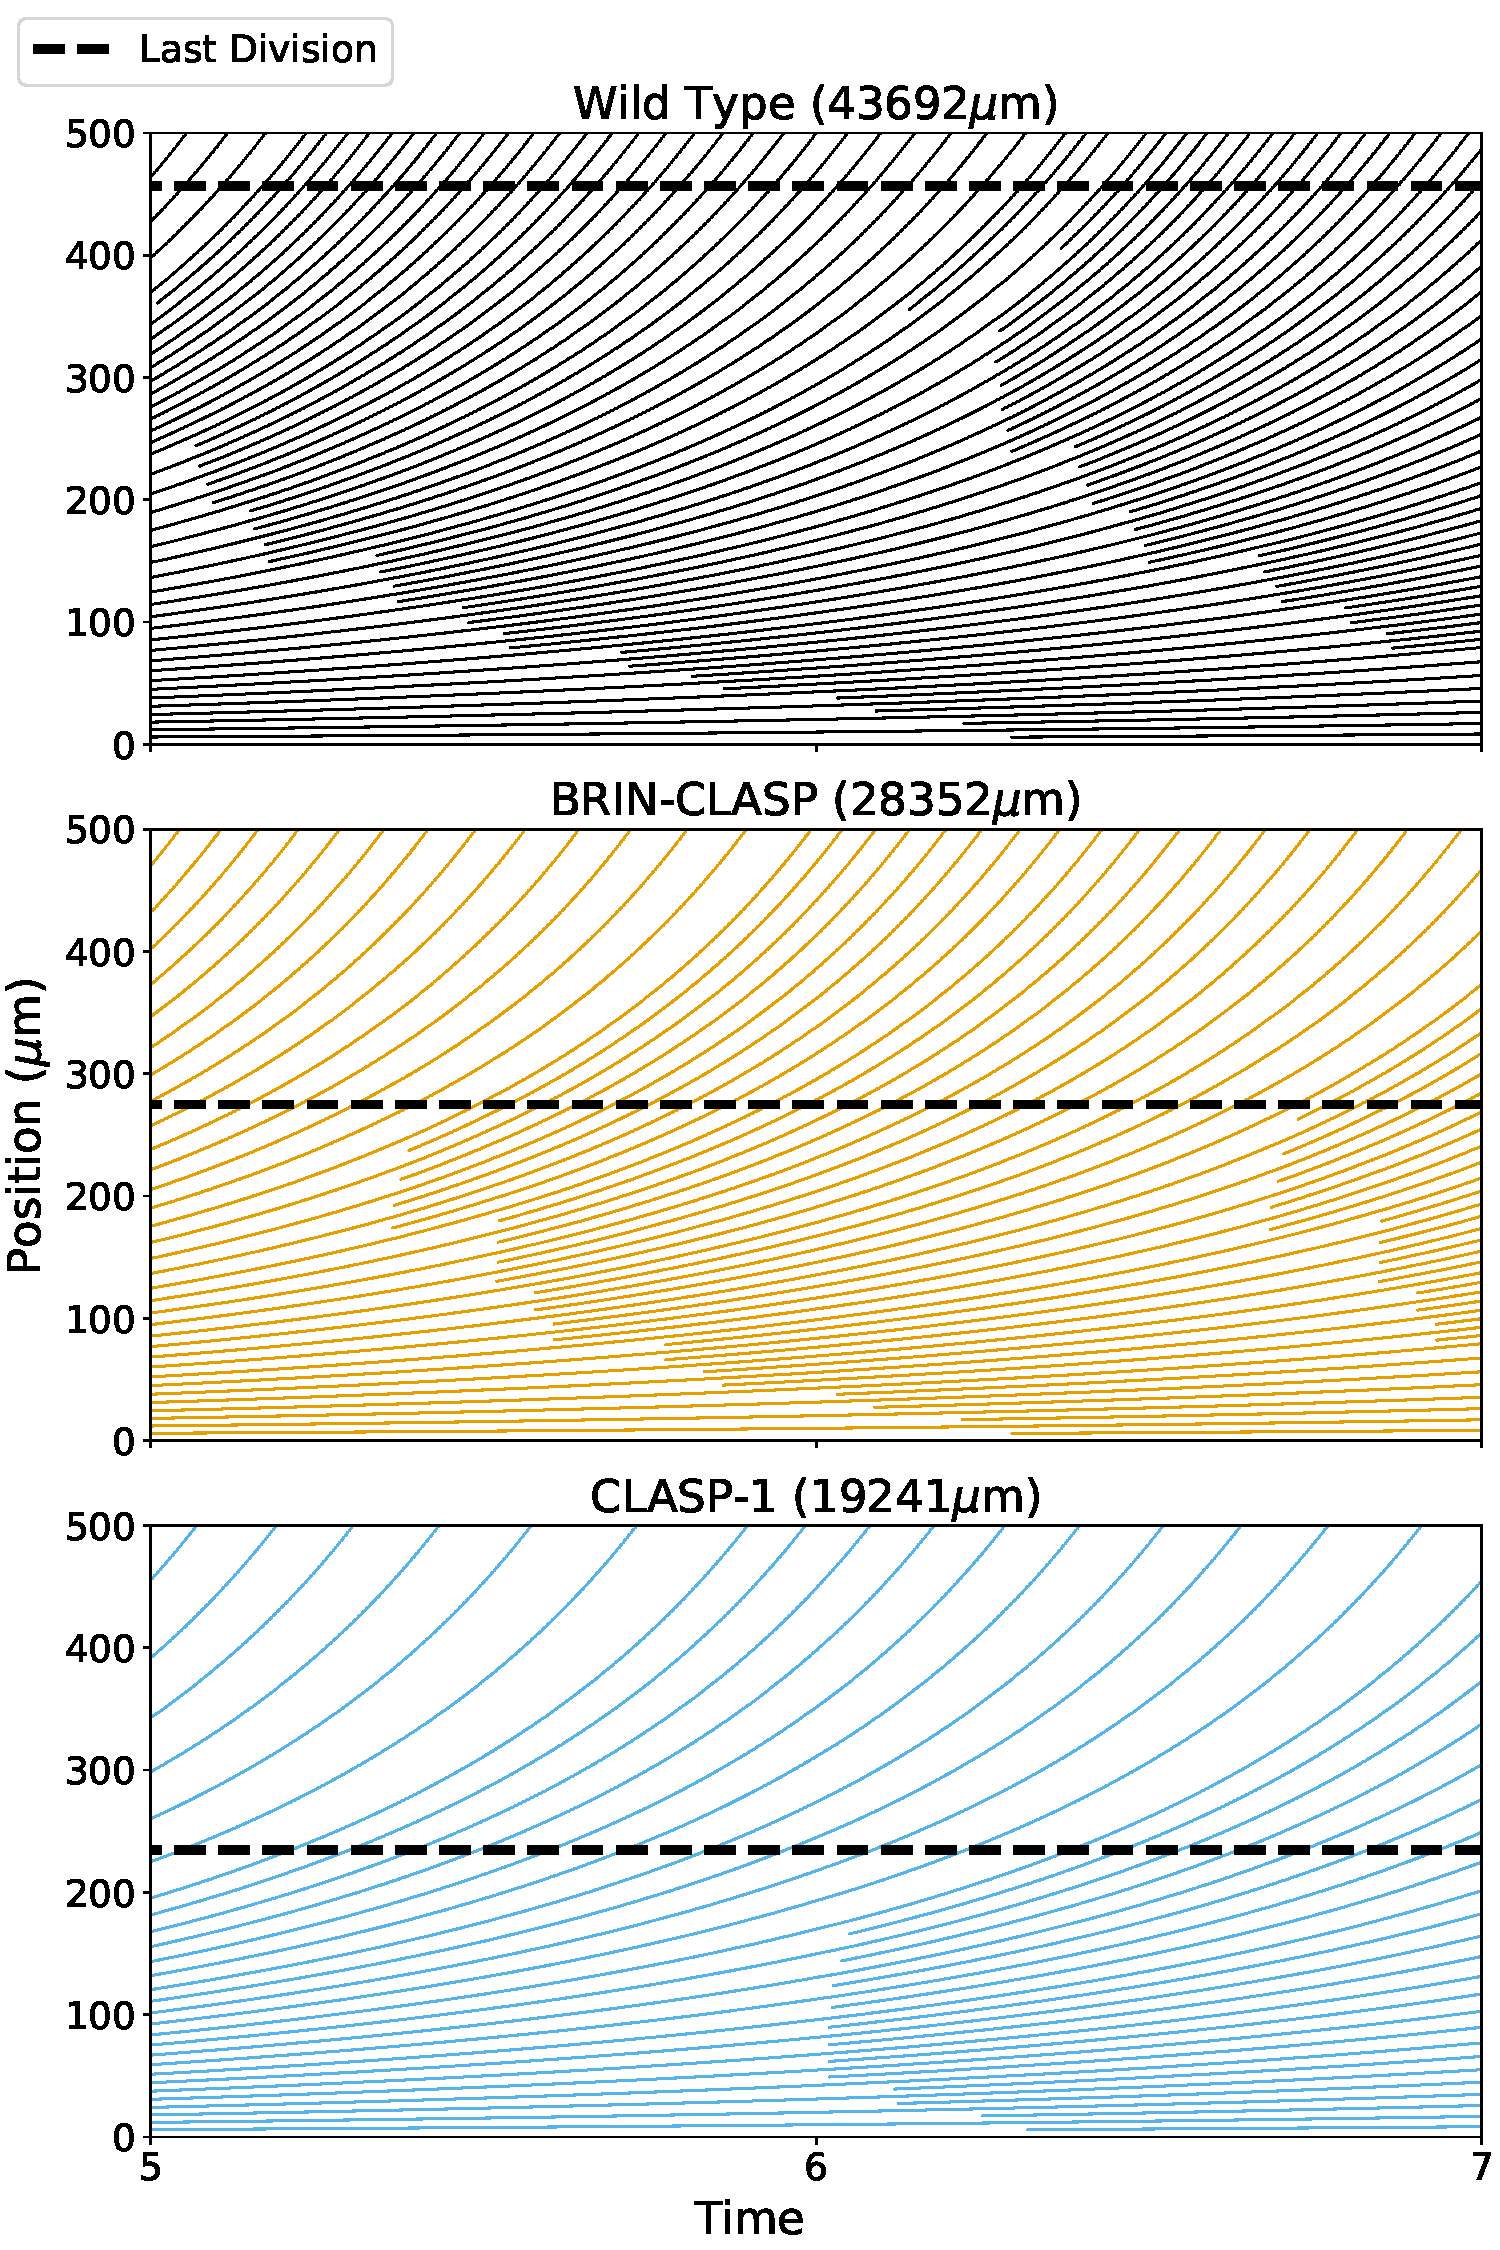
\includegraphics[height=480pt]{column-modified-profile.pdf}
  \caption{Cell column projection for the cell column model after modifying the division function to introduce a global maximum at an intermediate concentration of CLASP. The $x$-axis represents a (dimensionless) time variable while the $y$-axis represents distance from the quiescent centre in $\um$. The dotted black line is the highest position at which a division event occurred over the entire simulation. This point can be interpreted as the height of the division zone. Under this interpretation, the division zone of the wild type root is approximately twice the size of the division zone in the \emph{clasp-1} mutant and about $50\%$ larger than in the \emph{brinCLASPpro} mutant.}
  \label{column-modified-profile}
\end{figure}

\begin{figure}[!htp]
  \centering
  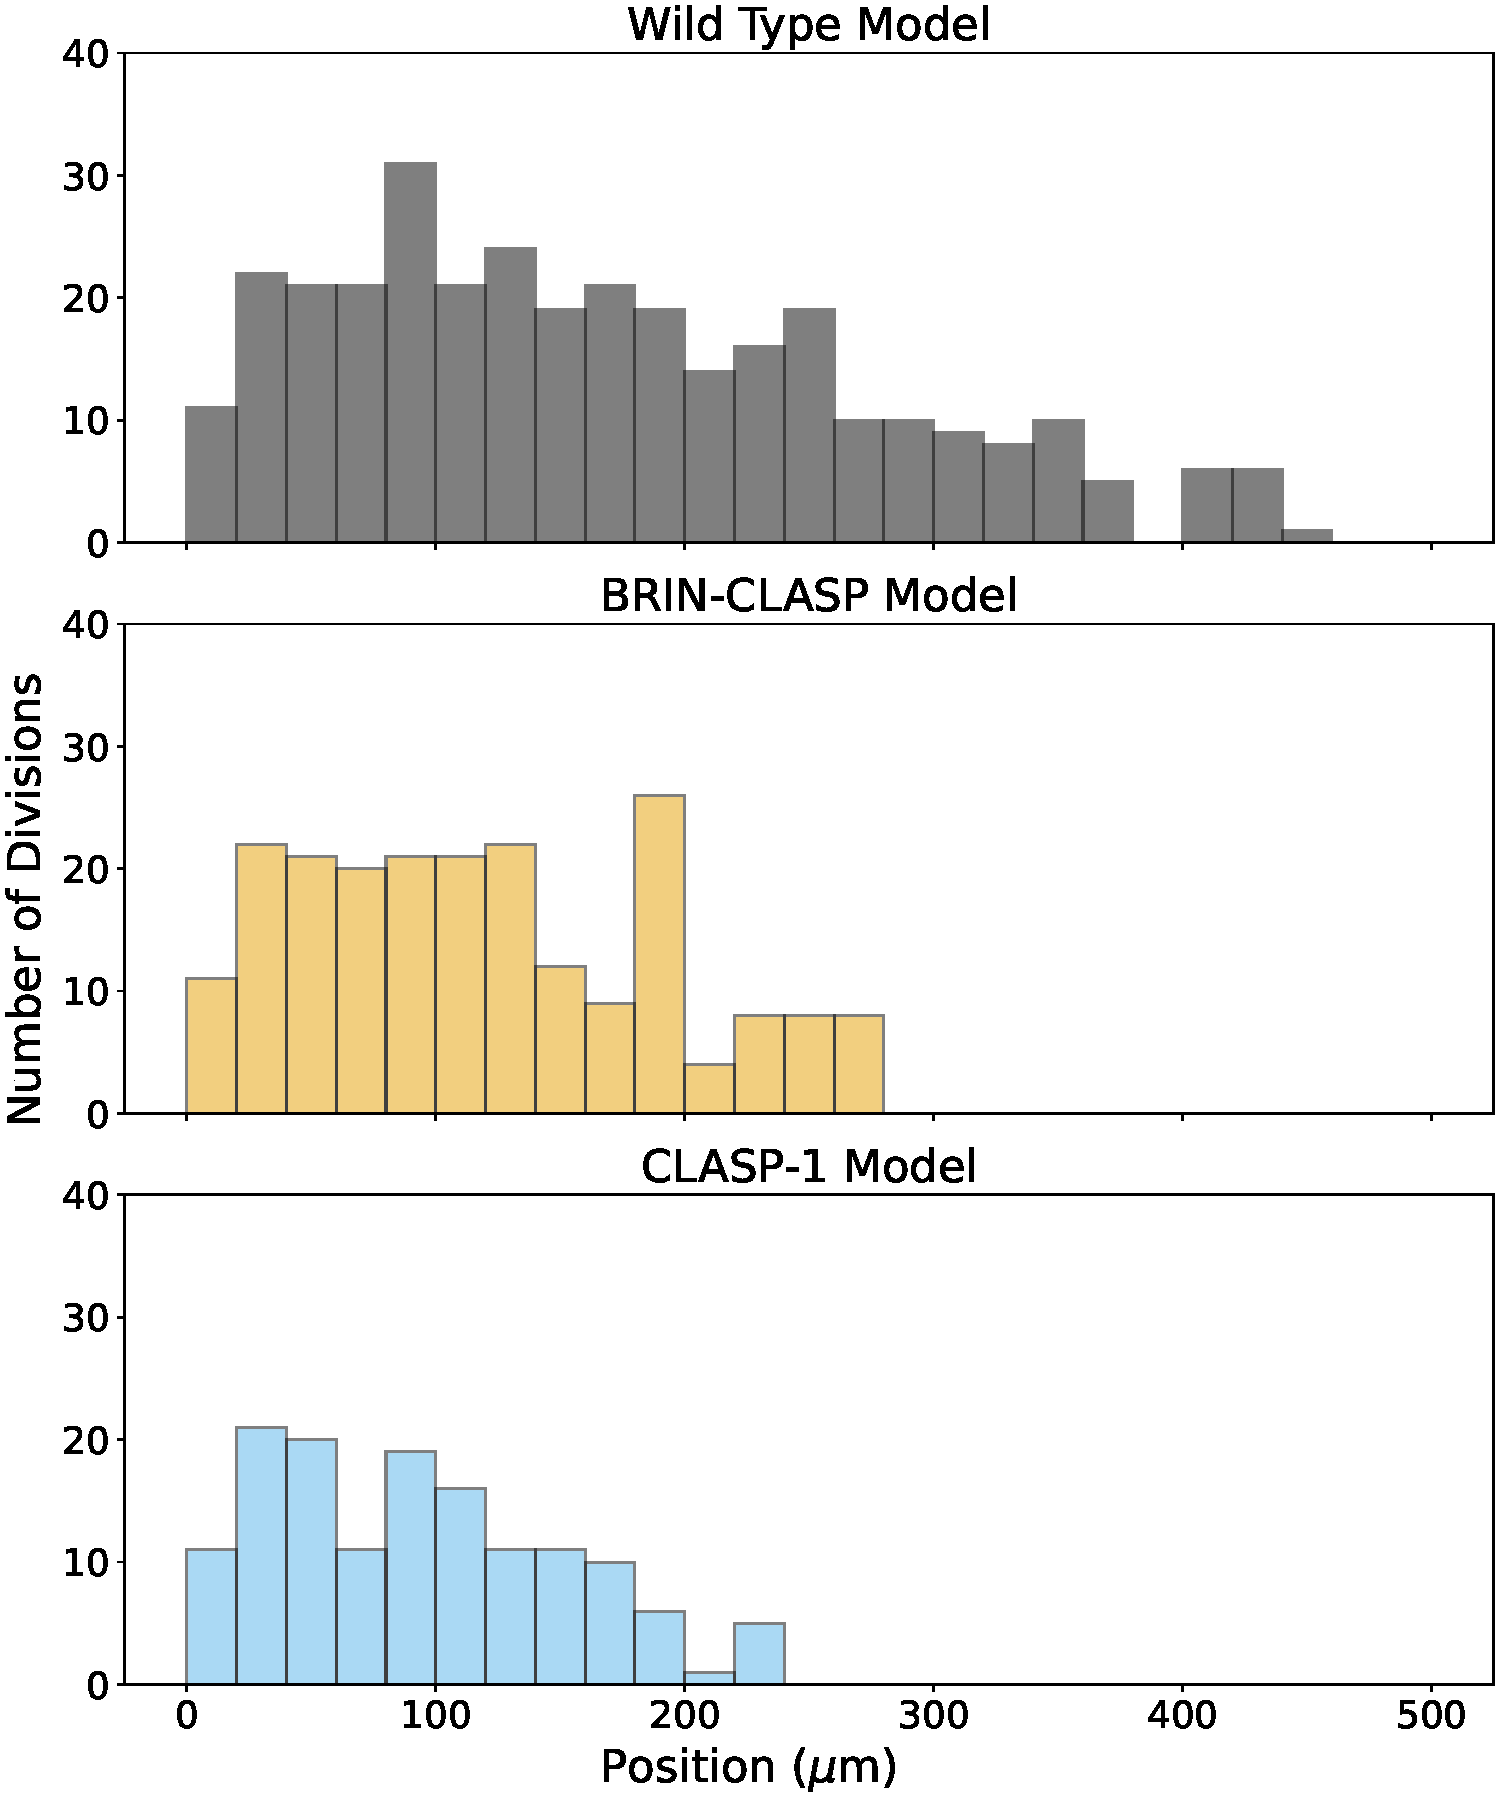
\includegraphics[width=\textwidth]{column-modified-histogram.pdf}
  \caption{Histogram of division locations for the cell column model after modifying the division function to introduce a global maximum at an intermediate concentration of CLASP. As in all previous figures, cell position is measured as distance from the quiescent centre in $\um$. The division locations have a unimodal distribution for all three genotypes, with some noise between the bins. In this model, there is a clear difference in the mean division position across the three genotypes, which reflects the smaller division zones in the \emph{brinCLASPpro} and \emph{clasp-1} mutants relative to the wild type.}
  \label{column-modified-histogram}
\end{figure}

\end{appendices}

\end{document}
